\chapter{Two-dimensional finite-volume methods}
\label{chp-2d-fv}
In Chapter \ref{chp-1d-fv}, we addressed the problem of solving the one-dimensional linear advection 
equation using the finite-volume method based on PPM.
In this Chapter, our focus shifts to solving the two-dimensional linear advection equation using the finite-volume method.
This step is crucial in our work since, as we will explore in Chapter \ref{chp-cs-fv},
solving the linear advection equation on the cubed-sphere relies on solving two-dimensional linear advection equations at each cube face,
with interpolation between adjacent panels, which are described in Chapter \ref{chp-cs-grids}.

A natural approach to develop a finite-volume method for the two-dimensional linear advection equation would involve extending PPM to two dimensions.
Indeed, \citet{rancic:1992} proposed a piecewise bi-parabolic extension of PPM using a semi-Lagrangian temporal discretization.
Further, this type of method can be extended to the cubed-sphere \citep{lauritzen:2010}.
However, this method suffers from a significant drawback—its computationally expensive nature.
As a popular alternative, dimension-splitting methods are often used, which replace the two-dimensional problem with a sequence of one-dimensional problems.
For example, we can solve the two-dimensional linear advection equation by solving a series of one-dimensional linear advection equations
using the PPM from Chapter \ref{chp-1d-fv}. Moreover, in principle, we can employ any numerical method that solves the one-dimensional linear advection equation.

A comparison between two-dimensional and dimension-splitting semi-Lagrangian schemes on a plane was investigated by \citet{chen:2017},
utilizing the PPM as the one-dimensional solver and distorted two-dimensional grids.
Their main conclusion was that dimension-splitting schemes are more sensitive to grid distortions, but they are computationally
cheaper and more accurate than two-dimensional methods, particularly when dealing with large CFL numbers.

The primary objective of this Chapter is to provide a comprehensive explanation of the dimension splitting method proposed by \citet{lin:1996}.
This method is currently utilized in the FV3 dynamical core and is applied to the two-dimensional linear advection equation using the one-dimensional
finite-volume schemes described in Chapter \ref{chp-1d-fv}.
To begin, similar to Chapter \ref{chp-1d-fv}, we start this Chapter with a review of the integral form of the two-dimensional
advection equation in Section \ref{sec-adv2d}. Following this, in Section \ref{sec:fv-2d}, we establish the framework for general two-dimensional finite-volume schemes.
Subsequently, the dimension splitting method is presented in Section \ref{sec-dsplit}, where we delve into its intricacies.
Finally, we showcase numerical experiments in Section \ref{sec-ds-exp} to illustrate the practical application of the dimension splitting approach.

\section{Two-dimensional advection equation in integral form}
\label{sec-adv2d}
\subsection{Notation}
\label{chp-adv2d-sec-not}
This Section is dedicated to extending the notation of Section \ref{chp-adv1d-sec-not}.
Based on definitions \ref{chp-adv1d-def-dxgrid} and \ref{chp-adv1d-def-dxtimegrid},
we introduce the concepts of a $(\Delta x,\Delta y)$-grid and $(\Delta x, \Delta y, \Delta t, \lambda)$ discretization.
Throughout this Chapter, we will use the notation $\Omega=[a,b]\times[c,d]$
and $\nu$ to represent a non-negative integer indicating the number of ghost cell layers in each boundary.
We also use the notations $\mathbb{R}^{N\times M}_{\nu}:=\mathbb{R}^{(N+2\nu)\times (M+2\nu)}$ and
$\mathbb{R}^{(N+1)\times M}_{\nu}:=\mathbb{R}^{(N+1+2\nu)\times (M+2\nu)}$,
$\mathbb{R}^{N\times (M+1)}_{\nu}:=\mathbb{R}^{(N+2\nu)\times (M+1+2\nu)}$.
\begin{definition}[$(\Delta x,\Delta y)$-grid]
	\label{chp-adv1d-def-2dgrid}
	Given $\Omega$ and positive real numbers $\Delta x$ and $\Delta y$ such that $\Delta x = (b-a)/N$, 
	$\Delta y = (d-c)/M$, for positive integers $N$ and $M$,
	we say that $\Omega_{\Delta x, \Delta y}=(\Omega_{ij})_{i=-\nu+1,\ldots,N+\nu}^{j=-\nu+1,\ldots,M+\nu}$
	is a $(\Delta x, \Delta y)$-grid for $\Omega$ if
    \begin{equation*}
	\Omega_{ij} = [x_{i-\frac{1}{2}}, x_{i+\frac{1}{2}}]\times [y_{j-\frac{1}{2}}, y_{j+\frac{1}{2}}] =
    [a+(i-1)\Delta x,a+i\Delta x]\times [c+(j-1)\Delta x,c+j\Delta x],
    \end{equation*}
	$\Delta x = x_{i+\frac{1}{2}}-x_{i-\frac{1}{2}}$, $\Delta y = y_{j+\frac{1}{2}}-y_{j-\frac{1}{2}}$.
	Each $\Omega_{ij}$ is called control volume or cell.
	The cell centroids $(x_i,y_j)$ are defined by
    \begin{align*}
       x_i = \frac{1}{2}(x_{i+\frac{1}{2}} + x_{i-\frac{1}{2}}), \quad y_j = \frac{1}{2}(y_{j+\frac{1}{2}} + y_{j-\frac{1}{2}}).
    \end{align*}
\end{definition}
\begin{remark}
If $1 \leq i \leq N$,$1 \leq j \leq M$, we refer to $(i,j)$ as an interior index;
otherwise, $(i,j)$ is considered a ghost cell index and we say the $\Omega_{ij}$ is a ghost cell.
\end{remark}
\begin{definition}[$(\Delta x,\Delta y,\Delta t, \lambda)$-discretization]
	\label{chp-adv1d-def-dxdytimegrid}
	Given $\Omega \times [0,T]$,
	and positive real numbers $\Delta x$ $\Delta y$ and $\Delta t$, we say that
	$(\Omega_{\Delta x, \Delta y}, {T}_{\Delta t})$
	is a $(\Delta x,\Delta y,\Delta t, \lambda)-$discretization of $\Omega \times [0,T]$ if
	$\Omega_{\Delta x, \Delta y}$ is a $(\Delta x,\Delta y)$
	grid for $\Omega$ and ${T}_{\Delta t}$ is a $\Delta t$-temporal
	grid for $[0,T]$, $\frac{\Delta t}{\Delta x} = \lambda$
	and  $\frac{\Delta t}{\Delta y} = \lambda$.
\end{definition}
\begin{remark}
	Whenever we mention a $(\Delta x,\Delta y)-$grid, or a $(\Delta x,\Delta y,\Delta t, \lambda)$-discretization,
	then $\Omega_{ij}$, $N$ and $M$ are implicitly defined.
\end{remark}
Next, we introduce the definitions of grid functions at cell centroids and C-grid functions. 
\begin{definition}[$(\Delta x,\Delta y)$-grid function]
	\label{chp-adv1d-rmk-2d-gridfunction1}
	For a $(\Delta x,\Delta y)$-grid, we say that $Q = (Q_{ij})_{i=-\nu+1,\ldots,N+\nu}^{j=-\nu+1,\ldots,M+\nu} \in \mathbb{R}^{N\times M}_{\nu}$ is a 
	$(\Delta x,\Delta y)$-grid function.
\end{definition}
\begin{definition}[$(\Delta x,\Delta y)$-C grid wind]
	\label{chp-adv1d-rmk-2d-gridfunction2}
	For a $(\Delta x,\Delta y)$-grid, we say that $(u,v)$ is a $(\Delta x,\Delta y)$-C grid wind if 
	$u = (u_{i+\frac{1}{2},j})_{i=-\nu,\ldots,N+\nu}^{j=-\nu+1,\ldots,M+\nu} \in \mathbb{R}^{(N+1) \times M}_{\nu}$, 
    $v = (v_{i,j+\frac{1}{2}})_{i=-\nu+1,\ldots,N+\nu}^{j=-\nu,\ldots,M+\nu} \in \mathbb{R}^{N \times (M+1)}_{\nu}$.
\end{definition}
Considering a function $q:\Omega\times[0,T] \to \mathbb{R}$,
a vector field $\boldsymbol{u}:\Omega\times[0,T] \to \mathbb{R}$, $\boldsymbol{u}=(u,v)$,
a $(\Delta x,\Delta y, \Delta t, \lambda)$-discretization
of $\Omega\times[0,T]$, we introduce the grid functions $q^n \in \mathbb{R}^{N\times M}_{\nu}$,
$u^n \in \mathbb{R}^{(N+1)\times M}_{\nu}$, $v^n \in \mathbb{R}^{N\times (M+1)}_{\nu}$. 
Here, ${q}^n_{ij} = {q}(x_i, y_j,t^{n})$, $u^n_{i+\frac{1}{2},j} = u(x_{i+\frac{1}{2}},y_j, t^n)$,
$v^n_{i,j+\frac{1}{2}} = u(x_i,y_{j+\frac{1}{2}}, t^n)$.
These grid functions represent the discrete values of $q$ and $\boldsymbol{u}$
at the cell centroids and edges, respectively,
for each time level $t^n$ (Figure \ref{chp-adv1d-sec1-grid1d-function}).
We shall also use the notations $q^n_{i+\frac{1}{2},j} = q(x_{i+\frac{1}{2}},y_j, t^n)$
and $q^n_{i,j+\frac{1}{2}} = q(x_i,y_{j+\frac{1}{2}}, t^n)$.
\begin{figure}[!htb]
	\centering
	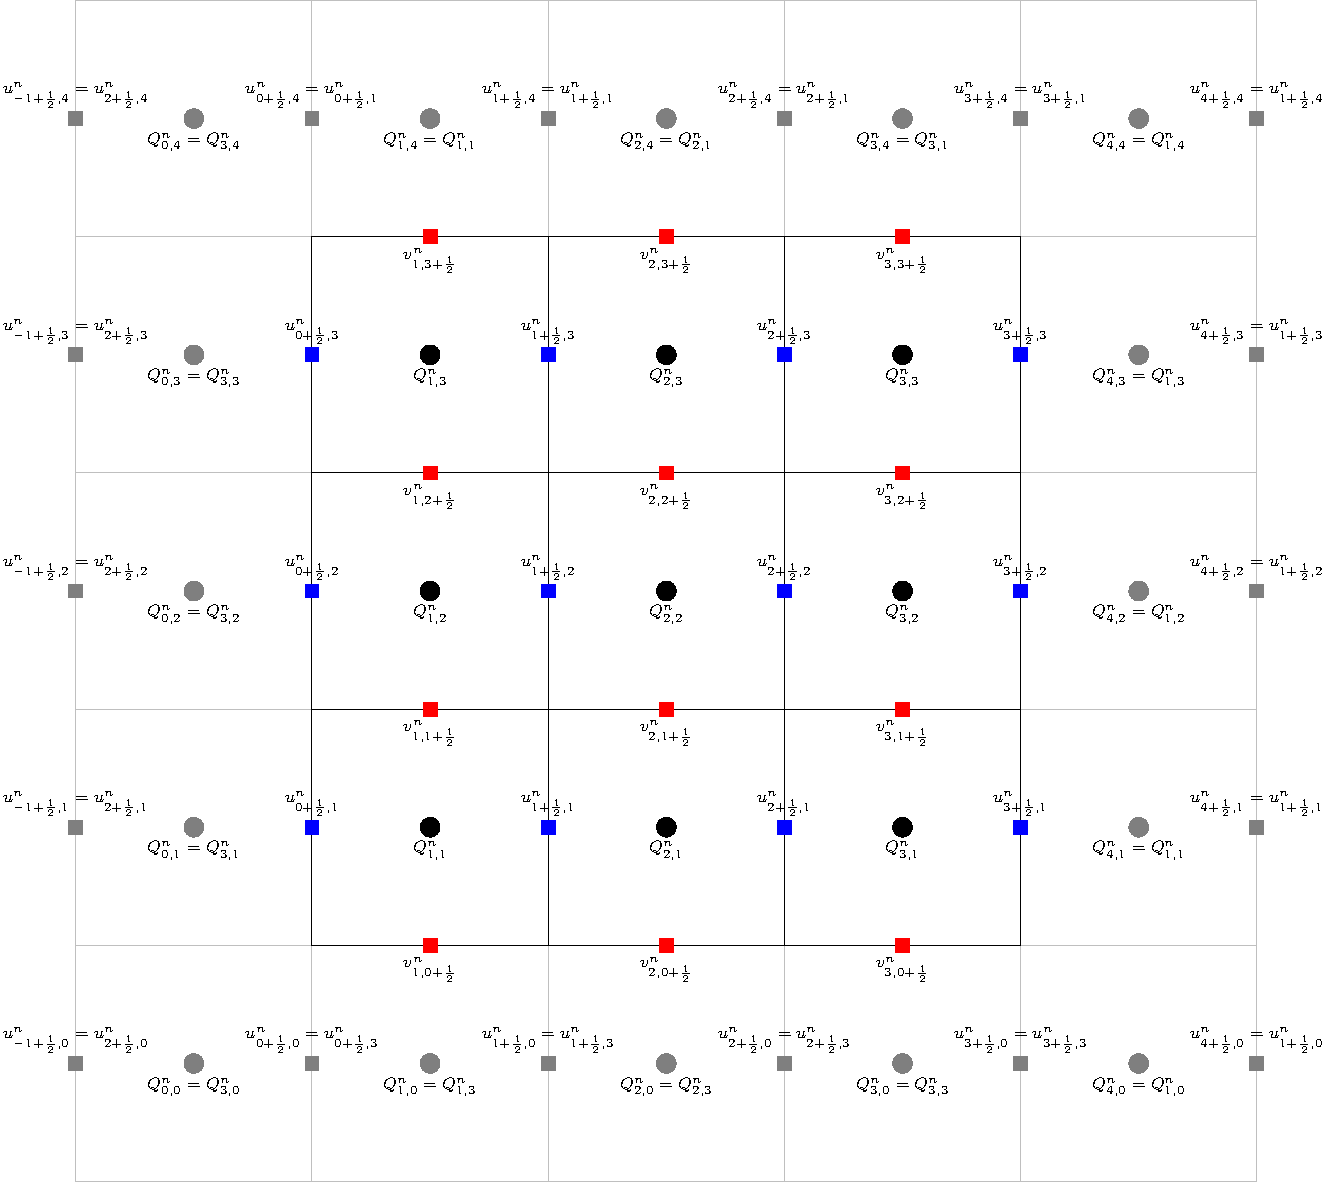
\includegraphics[width=1\linewidth]{2d_grid_function}
	\caption{Illustration of $(\Delta x, \Delta y)$-grid function $Q$ (black circles)
		and a $(\Delta x\Delta y)$-C grid wind $u$ (blue squares) and $v$ (red squares) and its ghost cell
		values (in gray) assuming biperiodicity.\label{chp-adv2d-sec1-grid2d-function}}
\end{figure}

We denote by $\nabla \cdot (q\boldsymbol{u})$ the divergence operator:
\begin{equation}
	\label{sec-adv2d:eqdiv}
	\nabla \cdot (q\boldsymbol{u})(x, y, t) =  
	[{\partial_x (uq)} + {\partial_y (vq)}](x, y, t).
\end{equation}
We recall that we say the $\boldsymbol{u}$ is \textbf{non-divergent} if $\nabla \cdot \boldsymbol{u}=0$.
We define the $(\Delta x, \Delta y)$-grid function $\delta^n$ as
the exact divergence of $q\boldsymbol{u}$ at the cell centers, namely
\begin{equation}
\label{2d-discrete-div}
\delta^n_{ij} = \nabla \cdot (\boldsymbol{u}q)(x_i,y_j,t^n).
\end{equation}
In this Chapter, our focus also lies on periodic grid functions.
We define a $(\Delta x, \Delta y)$-grid function $Q$ as periodic if it satisfies the following conditions:
\begin{align*}
    Q_{i,j} &= Q_{N+i,j}, \quad i=-\nu+1, \ldots, 0,  \quad &j = -\nu+1, \ldots, M+\nu,\\
    Q_{i,j} &= Q_{i-N,j}, \quad i=N+1, \ldots, N+\nu, \quad &j = -\nu+1, \ldots, M+\nu,\\
    Q_{i,j} &= Q_{i,M+j}, \quad j=-\nu+1, \ldots, 0,  \quad &i = -\nu+1, \ldots, N+\nu,\\
    Q_{i,j} &= Q_{i,j-M}, \quad j=M+1, \ldots, M+\nu, \quad &i = -\nu+1, \ldots, N+\nu.
\end{align*}
We use the notation $\mathbb{P}^{N \times M}_{\nu}$ represent the spaces of periodic $(\Delta x, \Delta y)$-grid functions.
Similarly, we define a $(\Delta x, \Delta y)$-grid wind $(u,v)$ as periodic if it meets the following requirements:
\begin{align*}
    u_{i-\frac{1}{2},j} &= u_{N+i+\frac{1}{2},j} , \quad i=-\nu, \ldots, -1,   \quad &j = -\nu+1, \ldots, M+\nu,\\
    u_{i+\frac{1}{2},j} &= u_{i+\frac{1}{2}-N,j} , \quad i=N+1, \ldots, N+\nu, \quad &j = -\nu+1, \ldots, M+\nu,\\
    u_{i+\frac{1}{2},j} &= u_{i+\frac{1}{2},M+j} , \quad i=-\nu, \ldots, N+1+\nu,   \quad &j = -\nu+1, \ldots, 0,\\
    u_{i+\frac{1}{2},j} &= u_{i+\frac{1}{2},j-M} , \quad i=-\nu, \ldots, N+1+\nu,   \quad &j = M+1, \ldots, M+\nu,\\
    v_{i,j-\frac{1}{2}} &= v_{i,M+j+\frac{1}{2}} , \quad j=-\nu, \ldots, -1,   \quad &i = -\nu+1, \ldots, N+\nu,\\
    v_{i,j+\frac{1}{2}} &= v_{i,j+\frac{1}{2}-M} , \quad j=M+1, \ldots, M+\nu, \quad &i = -\nu+1, \ldots, N+\nu,\\
    v_{i,j+\frac{1}{2}} &= v_{N+i,j+\frac{1}{2}} , \quad j=-\nu, \ldots, M+1+\nu,   \quad &i = -\nu+1, \ldots, 0,\\
    v_{i,j+\frac{1}{2}} &= c_{i-N,j+\frac{1}{2}} , \quad j=-\nu, \ldots, N+1+\nu,   \quad &i = N+1, \ldots, N+\nu.\\
\end{align*}
In this case, we use the notation $u \in \mathbb{P}^{(N+1) \times M}_{\nu}$, 
$v \in \mathbb{P}^{N \times (M+1)}_{\nu}$.

For a grid function $Q$ we also use the notations:
\begin{align*}
Q_{\times,j} &:= (Q_{-\nu+1,j}, \ldots, Q_{N+\nu,j}) \in \mathbb{R}^N_{\nu},\\
Q_{i,\times} &:= (Q_{i,-\nu+1}, \ldots, Q_{i,M+\nu}) \in \mathbb{R}^M_{\nu}.
\end{align*}
Given $Q = (Q_{ij})\in \mathbb{P}^{N \times M}_{\nu, P}$, we define the $p$-norm by
\begin{equation}
	\label{chp-adv2d-pnorm}
	\|Q\|_{p,\Delta x \times \Delta y}=
	\begin{cases}
		\bigg( \sum_{i=1}^{N} \sum_{j=1}^{M}|Q_{ij}|^p \bigg)^{\frac{1}{p}} & \text{if } 1\leq p < \infty,\\
		\max_{i=1, \ldots, N,j=1,\ldots,M}{|Q_{ij}|} & \text{otherwise }.
	\end{cases}
\end{equation}
We also introduce the centered difference notation:
\begin{align}
	\label{sec-adv2d:eq6}
	\delta_x {h}(x_i,y, t) = 
	{h}(x_{i+\frac{1}{2}}, y, t) - 
	{h}(x_{i-\frac{1}{2}}, y, t), \\
	\delta_y {h}(x, y_j,t) = 
    {h}(x, y_{j+\frac{1}{2}},t) - 
    {h}(x, y_{j-\frac{1}{2}},t),
\end{align}
for any function $h: \Omega \times [0,T] \to \mathbb{R}$.
Additionally, we introduce the average value of $q$ in the control volume
$\Omega_{ij}$ at time $t$, denoted as ${Q}_{ij}(t)$, defined by:
\begin{equation}
	\label{chp-adv2d-sec1-not2}
	{Q}_{ij}(t) = \frac{1}{\Delta x \Delta y}
	\int_{x_{i-\frac{1}{2}}}^{x_{i+\frac{1}{2}}} \int_{y_{j-\frac{1}{2}}}^{y_{j-\frac{1}{2}}} {q}(x,y,t) \,dx.
\end{equation}
Moreover, we define the $(\Delta x, \Delta y)$-grid function of average values as $Q(t) = (Q_{ij}(t))_{i=-\nu+1,\ldots,N+\nu}^{j=-\nu+1,\ldots,M+\nu}$.

For the consideration of periodic boundary conditions, we can define spaces of periodic functions over 
the interval $\Omega$ as follows:
\begin{align*}
	\mathcal{S}_P(\Omega) &= \{q:\mathbb{R}^2\times[0,+\infty[\to \mathbb{R}: q(x+b-a,y+d-c,t)=q(x,y,t), \quad \forall x,y \in \mathbb{R}, \quad t\geq0\}.
\end{align*}
Similarly, the space of $k$-times periodically differentiable functions $\mathcal{C}_P^k(\Omega)$ can be defined as:
\begin{align*}
	\mathcal{C}_P^k(\Omega) &= \mathcal{S}_P(\Omega) \cap \mathcal{C}^k(\mathbb{R}^2\times[0,\infty[),
\end{align*}
where $\mathcal{C}^k(\mathbb{R}^2\times[0,+\infty[)$ denotes the space of functions that are $k$ 
times continuously differentiable in both the spatial and temporal variables.
In summary, $\mathcal{S}_P(\Omega)$ represents the space of periodic functions, and $\mathcal{C}_P^k(\Omega)$
represents the space of $k$-times periodically differentiable functions over $\Omega$ subject to periodic boundary conditions.

\subsection{The 2D advection equation}
Let us consider a  velocity field given by $\boldsymbol{u}=(u,v)$, where
$u$ is the velocity in $x$-direction and $v$ is the velocity in $x$ and $y$ direction
and $u,v \in \mathcal{C}^1_P(\Omega)$.
The two-dimensional advection equation in its differential form in 
a domain $\Omega$ associated to the velocity field or wind $\boldsymbol{u}$ 
and assuming biperiodic boundary conditions is given by:
\begin{equation}
	\label{sec-adv2d:eq1}
	\begin{cases}
		[{\partial_t q} + {\partial_x (uq)} +  {\partial_y (vq)}](x, y, t)
		= 0, \quad \forall (x,y,t) \in \mathbb{R}^2\times ]0, +\infty[,\\
		{q}(a, y, t) = {q}(b, y, t), \quad \forall y \in [c,d],  \quad \forall t\geq 0, \\
		{q}(x, c, t) = {q}(x, d, t), \quad \forall x \in [a,b],  \quad \forall t\geq 0, \\
		q_0(x) = q(x,y,0), \quad \forall (x,y) \in \Omega.
	\end{cases}
\end{equation} 
A classical or strong solution to the two-dimensional advection equation is a 
$\mathcal{C}^1_P{(\Omega)}$ function ${q}$ satisfying Equation \eqref{sec-adv2d:eq1}.
As we did in Section \ref{chp-adv1d-sec1}, our goal is to deduce an
integral form of Equation \eqref{sec-adv2d:eq1}.
Thus, let us consider  $[x_1,x_2] \times [y_1, y_2]
\subset \Omega$ and $[t_1,t_2] \subset [0, +\infty[$.
Integrating Equation $\eqref{sec-adv2d:eq1}$ over 
$[x_1,x_2] \times [y_1, y_2]$ yields:
\begin{align}
	\label{sec-adv2d:eq2}
	\frac{d}{d t} \bigg(\int_{x_1}^{x_2} \int_{y_1}^{y_2}
	{q}(x, y, t) \,dx \,dy \bigg)=
	&-\int_{y_1}^{y_2} \bigg({(uq)}(x_2, y, t)
	-{(uq)}(x_1, y, t) \bigg) \,dy \\ \nonumber
	&-\int_{x_1}^{x_2} \bigg({(vq)}(x, y_2, t)
	-{(vq)}(x, y_1, t) \bigg) \,dx.
\end{align}
Integrating Equation \eqref{sec-adv2d:eq2} over the time interval $[t_1,t_2]$, 
we have:
\begin{align}
	\label{sec-adv2d:eq3}
	\int_{x_1}^{x_2} \int_{y_1}^{y_2}
	{q}(x, y, t_{n+1}) \,dx \,dy = &\int_{x_1}^{x_2} \int_{y_1}^{y_2}
	{q}(x, y, t_n) \,dx \,dy \\ \nonumber
	&-\int_{t_1}^{t_2} \int_{y_1}^{y_2} \bigg({(uq)}(x_2, y, t)
	-{(uq)}(x_1, y, t) \bigg) \,dy \,dt\\ \nonumber
	&-\int_{t_1}^{t_2} \int_{x_1}^{x_2} \bigg({(vq)}(x, y_2, t)
	-{(vq)}(x, y_1, t) \bigg) \,dx \,dt.
\end{align}
Equation \eqref{sec-adv2d:eq3} is the integral form of Equation 
\eqref{sec-adv2d:eq1}. We say that ${q}$ is a weak
solution to the advection equation \eqref{sec-adv2d:eq1} if ${q}$
satisfies the integral form \eqref{sec-adv2d:eq3}, 
$\forall [x_1,x_2]\times[y_1,y_2] \subset \Omega^{\mathrm{o}}$ and 
$\forall [t_1,t_2] \subset [0,+\infty[$.
We summarize the weak version of Equation \eqref{sec-adv2d:eq1} in Problem \eqref{chp-adv2d-sec2-prob1}.
\begin{prob}
	\label{chp-adv2d-sec2-prob1}
	Given an initial condition ${q}_0$ and
	a velocity function $\boldsymbol{u} = (u,v)$
 	we would like to find a weak solution ${q}$
	of the two-dimensional advection equation in its integral form:
	\begin{align*}
		\int_{x_1}^{x_2} \int_{y_1}^{y_2}
		{q}(x, y, t) \,dx \,dy = &\int_{x_1}^{x_2} \int_{y_1}^{y_2}
		{q}(x, y, t) \,dx \,dy \\ \nonumber
		&-\int_{t_1}^{t_2} \int_{y_1}^{y_2} \bigg({(uq)}(x_2, y, t)
		-{(uq)}(x_1, y, t) \bigg) \,dy \,dt\\ \nonumber
		&-\int_{t_1}^{t_2} \int_{x_1}^{x_2} \bigg({(vq)}(x, y_2, t)
		-{(vq)}(x, y_1, t) \bigg) \,dx \,dt.
	\end{align*}
	$\forall [x_1, x_2]\times [y_1, y_2] \times[t_1, t_2] \subset \Omega \times[0,T]$, 
	and ${q}(x, y, 0) = {q}_0(x, y)$, $\forall (x, y) \in \Omega$,
   ${q}(a, y, t) = {q}(b, y, t), \quad \forall y \in [c,d],  \quad \forall t\geq 0,$
   ${q}(x, c, t) = {q}(x, d, t), \quad \forall x \in [a,b],  \quad \forall t\geq 0.$
\end{prob}
Similarly to Section \ref{chp-adv1d-sec1}, Equation \eqref{sec-adv2d:eq1} and Problem \eqref{chp-adv2d-sec2-prob1} are equivalent
when ${q}, \boldsymbol{u} \in \mathcal{C}^1_P{(\Omega)}$.
For Problem \ref{chp-adv2d-sec2-prob1}, the total mass in $\Omega$ is defined by: 
\begin{equation}
	{M}_{\Omega}(t) = \int_{\Omega} {q}(x,y,t) \,dx \,dy , \quad \forall t \in [0,T],
\end{equation}
and is conserved within time: 
\begin{equation}
	{M}_{\Omega}(t) = {M}_{\Omega}(0), \quad \forall t \in [0,T].
\end{equation}
Considering a $(\Delta x, \Delta y, \Delta t, \lambda)$ discretization of $D = \Omega \times [0,T]$ and
substituting $t_1, t_2, x_1, x_2, y_1$ and $y_2$ by 
$t_{n}, t_{n+1}, x_{i-\frac{1}{2}}, x_{i+\frac{1}{2}}, y_{j-\frac{1}{2}}, y_{j+\frac{1}{2}}$,
respectively, in Equation \eqref{sec-adv2d:eq3}, we obtain:
\begin{align}
	\label{sec-adv2d:eq5}
	{Q}_{ij}(t_{n+1})  = {Q}_{ij}(t_{n})
	&- \frac{\Delta t}{\Delta x \Delta y}
	\delta _x \bigg( \frac{1}{\Delta t}
	\int_{t_1}^{t_2} \int_{y_{j-\frac{1}{2}}}^{y_{j+\frac{1}{2}}} 
	{(uq)}(x_{i}, y, t)
	\,dy \,dt \bigg) \\ \nonumber
	&- \frac{\Delta t}{\Delta x \Delta y}
	\delta _y \bigg( \frac{1}{\Delta t}
	\int_{t_1}^{t_2} \int_{x_{i-\frac{1}{2}}}^{x_{i+\frac{1}{2}}} 
	{(vq)}(x, y_{j}, t)
	\,dx \,dt \bigg),
\end{align}
where we are using the centered finite-difference notation.
Now we can define a discretized version of Problem \ref{chp-adv2d-sec2-prob1} as Problem \ref{chp-adv2d-sec2-prob2}.
\begin{prob}
	\label{chp-adv2d-sec2-prob2}
	Assume the framework of Problem \ref{chp-adv2d-sec2-prob1}
	and consider a $(\Delta x, \Delta y, \Delta t, \lambda)$-discretization of $\Omega\times [0,T]$.
	Since we are in the framework of Problem \ref{chp-adv2d-sec2-prob1}, it follows that:
	\begin{align*}
		{Q}_{ij}(t_{n+1})  = {Q}_{ij}(t_{n})
		&- {\lambda}
		\delta _x \bigg( \frac{1}{\Delta t \Delta y}
		\int_{t^n}^{t^{n+1}} \int_{y_{j-\frac{1}{2}}}^{y_{j+\frac{1}{2}}} 
		{(uq)}(x_{i}, y, t)
		\,dy \,dt \bigg) \\ \nonumber
		&- {\lambda}
		\delta _y \bigg( \frac{1}{\Delta t \Delta x}
		\int_{t^n}^{t^{n+1}} \int_{x_{i-\frac{1}{2}}}^{x_{i+\frac{1}{2}}} 
		{(vq)}(x, y_{j}, t)
		\,dx \,dt \bigg),
	\end{align*}
	where ${Q}_{ij}(t) = \frac{1}{\Delta x \Delta y}
	\int_{x_{i-\frac{1}{2}}}^{x_{i+\frac{1}{2}}} 
	\int_{y_{j-\frac{1}{2}}}^{y_{j+\frac{1}{2}}} {q}(x,y,t) \,dx \,dy$.
	Our problem now consists of finding the values ${Q}_{ij}(t_{n})$, 
	$\forall i = 1, \ldots, N$, $\forall j = 1, \ldots, M$, $\forall n = 0, \ldots, N_T-1$,
    given the initial values ${Q}_{ij}(0)$, $\forall i = 1, \ldots N$, $\forall j = 1, \ldots, M$.
    In other words, we aim to find the average values of ${q}$ in each control volume $\Omega_{ij}$ at the specified time instances.
\end{prob}
It is important to note that no approximations have been made in Problems \eqref{chp-adv2d-sec2-prob1} and \eqref{chp-adv2d-sec2-prob2}. 

\section{The finite-volume approach}
\label{sec:fv-2d}
Finally, we define the 2D-FV scheme problem as follows in Problem \ref{chp-adv2d-sec2-prob3}.
\begin{prob}[2D-FV scheme]
	\label{chp-adv2d-sec2-prob3}
	Assume the framework defined in Problem \ref{chp-adv2d-sec2-prob2}.
	The finite-volume approach of Problem \ref{chp-adv2d-sec2-prob1}
	consists of a finding a scheme of the form:
	\begin{align}
		\label{chp-adv2d-2dfv}
		{Q}_{ij}^{n+1} =  {Q}_{ij}^{n} - {\lambda} \delta_i {F}_{ij}^{n} - {\lambda} \delta_j {G}_{ij}^{n},
		\\ \nonumber \quad \forall i = 1, \ldots, N, \quad \forall j = 1, \ldots, M,
		\quad \forall n = 0, \ldots, N_T-1,
	\end{align}
	where $ \delta_i F_{ij}^n =
    {F}_{i+\frac{1}{2},j}^{n} 
    - {F}_{i-\frac{1}{2},j}^{n}$,
    $ \delta_j G_{ij}^n =
    {G}_{i,j+\frac{1}{2}}^{n} 
    - {G}_{i,j-\frac{1}{2}}^{n}$ 
    and ${Q}^{n}\in \mathbb{P}^{N\times M}_{\nu}$ is intended to be an approximation
	of ${Q}(t_{n})\in \mathbb{P}^{N\times M}_{\nu}$ in some sense. We define ${Q}_{ij}^{0} = {Q}_{ij}(0)$ or
	${Q}_{ij}^{0} = {q}^0_{ij}$.
    
    The term ${F}_{i+\frac{1}{2}, j}^{n}$ is known as numerical flux in the 
    $x$ direction and it approximates
	$\frac{1}{\Delta t \Delta y}\int_{t_n}^{t_{n+1}} 
    \int_{y_{j-\frac{1}{2}}}^{y_{j+\frac{1}{2}}} 
    (uq)(x_{i+\frac{1}{2}}, y, t) \,dy \,dt $,
    $\forall i = 0, 1, \ldots, N$, and 
	${G}_{i, j+\frac{1}{2}}^{n}$ is known as numerical flux in the 
    $y$ direction and it approximates
	$\frac{1}{\Delta t \Delta x}\int_{t_n}^{t_{n+1}}  
    \int_{x_{i-\frac{1}{2}}}^{x_{i+\frac{1}{2}}}
    (vq)(x, y_{j+\frac{1}{2}}, t) \,dx \,dt $,
    $\forall j = 0, 1, \ldots, M$,
	or, in other words, they estimate the time-averaged
    fluxes at the control volume $\Omega_{ij}$ boundaries.
\end{prob}
\begin{remark}
For Problem \ref{chp-adv2d-sec2-prob3}, we define the CFL number in the $x$ and $y$ direction
by $\max \{{|u_{i+\frac{1}{2},j}^n}|\}\frac{\Delta t}{\Delta x}$ and 
$\max \{ {|v_{i,j+\frac{1}{2}}^n}|\}\frac{\Delta t}{\Delta y}$, respectively.
The CFL number is maximum between these numbers and we say that the CFL condition is
satisfied if the CFL number is less than one. 
\end{remark}
For a 2D-FV the discrete total mass at the time-step $n$ is given by
\begin{equation*}
	M^n =  \Delta x \Delta y \sum_{i=1}^N \sum_{j=1}^M Q_{ij}^n.
\end{equation*}
Therefore, the discrete total mass is constant for a 2D-FV scheme,
which follows from a straightforward computation:
\begin{align*}
	M^{n+1} &=  \Delta x \sum_{i=1}^N  \sum_{j=1}^M Q_{ij}^{n+1} 
	= M^{n} - \Delta t  \sum_{i=1}^N  \sum_{j=1}^M (F^n_{i+\frac{1}{2},j}- F^n_{i-\frac{1}{2},j})
	 		 - \Delta t  \sum_{i=1}^N  \sum_{j=1}^M (G^n_{i,j+\frac{1}{2}}- G^n_{i,j-\frac{1}{2}})\\
	&= M^{n} - \Delta t \sum_{j=1}^M (F^n_{N+\frac{1}{2},j}- F^n_{\frac{1}{2},j})
			 - \Delta t \sum_{i=1}^N (G^n_{i,M+\frac{1}{2}}- G^n_{i,\frac{1}{2}})
	= M^{n},
\end{align*}
where we are using that $F^n_{N+\frac{1}{2},j} = F^n_{\frac{1}{2},j}$,
$G^n_{i,M+\frac{1}{2}} = G^n_{i,\frac{1}{2}}$ since we are assuming bi-periodic boundary
conditions.

As we mentioned in Problem \ref{chp-adv2d-sec2-prob3}, the initial condition may be assumed as $q_{ij}^0$ or $Q_{ij}(0)$. 
For two-dimensional simulations, we are going to assume  $q_{ij}^0$ as initial data to avoid the computation of integrals.
Furthermore, the errors will be calculated using the values $q_{ij}^n$ instead of $Q_{ij}(t_n)$.
Similarly to Proposition \ref{prop-bound-centroid}, we have that the centroid value approximates the average value
with second order, as Proposition \ref{prop-bound-centroid-2d} shows.
\begin{prop}
	\label{prop-bound-centroid-2d}
	If $q \in \mathcal{C}^2$, then $|Q_{ij}(t^n)-q_{ij}^n| = C_1 \Delta x^2 + C_2 \Delta x \Delta y + C_3 \Delta y^2$, where 
	$C_1$, $C_2$ and $C_3$ are constants.
\end{prop}
\begin{proof}
	Just apply Theorem \ref{prop-bound-midpoint2d} for the function $q(x,y,t^n)$.	
\end{proof}

In order to check the consistency of 2D-FV, it is useful to use the notion of discrete divergence.
\begin{definition}[Discrete divergence]
	\label{chp-adv2d-def-div}
	For Problem \ref{chp-adv2d-sec2-prob3}, we define the discrete divergence as a 
    $(\Delta x, \Delta y)$-grid function $\mathbb{D}^n(Q^n,u^n,v^n) \in \mathbb{P}^{N\times M}_{\nu}$
	given by:
	\begin{equation}
		\label{chp-adv2d-def-div-eq}
		\mathbb{D}_{ij}^n(Q^n,u^n,v^n)=  \frac{1}{\Delta t}
        \bigg(\frac{\delta_i {F}_{ij}^{n}}{\Delta x} + \frac{\delta_j {G}_{ij}^{n}}{\Delta y} \bigg), 
        \quad i = 1, \ldots, N, \quad j=1, \ldots,M.
	\end{equation}
\end{definition}
With the aid of the discrete divergence, we may rewrite Equation \eqref{chp-adv2d-2dfv} as:
\begin{align}
    \label{chp-adv2d-2dfv-div}
    {Q}^{n+1} =  {Q}^{n} - \Delta t \mathbb{D}^n(Q^n,u^n,v^n),
\end{align}
Notice that if we replace  $Q^n$ by the exact solution $Q(t^n)$ in Equation \eqref{chp-adv2d-2dfv-div}, we have
\begin{align}
    \label{chp-adv2d-div-tau}
    {Q}(t^{n+1}) =  {Q}(t^{n}) - \Delta t \mathbb{D}^n(Q(t^n),u^n,v^n) - \Delta t \tau^n,
\end{align}
where $\tau^n \in \mathbb{P}^{N\times M}_{\nu}$ is the local truncation error (LTE).
Rearranging the terms of Equation \eqref{chp-adv2d-div-tau}, we obtain:
\begin{align}
    \label{chp-adv2d-div-tau2}
    \tau^n =  \frac{{Q}(t^{n+1}) - {Q}(t^{n})}{\Delta t} - \mathbb{D}^n(Q(t^n),u^n,v^n).
\end{align}
We define the consistency of the 2D-FV scheme as follows.
\begin{definition}[Consistency]
	\label{chp-adv2d-def-cons}
	Let us consider the framework of Problem \ref{chp-adv2d-sec2-prob3}.
	A 2D-FV scheme is said to be consist in the $p$-norm if for any sequence of
	$(\Delta x^{(k)},\Delta y^{(k)}, \Delta t^{(k)},\lambda)$-discretizations, 
	$k \in \mathbb{N}$, with
    $\lim_{k\to \infty }{\Delta x^{(k)}} =\lim_{k\to \infty }{\Delta y^{(k)}}= \lim_{k\to \infty }{\Delta t^{(k)}} = 0$, we have:
	\begin{equation*}
		\lim_{k \to \infty}\bigg[ {\max_{1\leq n\leq N_T^{(k)}}}{\|\tau^n\|_{p,\Delta x^{(k)} \times \Delta y^{(k)}}} \bigg] = 0,
	\end{equation*}
	and it is said to be consistent with order $d$ in the $p-$norm if
	\begin{equation*}
		{\max_{1\leq n\leq N_T^{(k)}}}{\|\tau^n\|_{p,\Delta x^{(k)} \times \Delta y^{(k)}}} = \mathcal{O}(\Delta x^d).
	\end{equation*}
\end{definition}
The relationship between consistency and convergence is explained in Section \ref{chp-adv2d-CCS}.
If $q$ satisfies Equation \eqref{sec-adv2d:eq1}, it can be observed that consistency is equivalent to the following:
\begin{equation*}
	{\max_{1\leq n\leq N_T^{(k)}}}{\|\delta^n - \mathbb{D}^n(Q^n,u^n,v^n)\|_{p,\Delta x^{(k)} \times \Delta y^{(k)}}} = \mathcal{O}(\Delta x^d),
\end{equation*}
where $\delta^n \in \mathbb{P}^{N\times M}_{\nu}$ is defined in Equation \eqref{2d-discrete-div}.
Therefore, we can determine whether a 2D-FV scheme is consistent by comparing the discrete divergence to the exact divergence.

\section{Dimension splitting}
\label{sec-dsplit}
This Section aims to demonstrate how a 2D-FV scheme, such as the one presented in Problem \ref{chp-adv2d-sec2-prob3},
can be constructed using 1D-FV schemes through a technique known as dimension splitting.
Before introducing the dimension splitting scheme proposed by \citet{lin:1996},
it is helpful to examine general operator splitting schemes,
as the dimension splitting technique is a specific instance of operator splitting methods.

For a given time interval $[0,T]$, we utilize a $\Delta t$-temporal grid. Let us consider the abstract Cauchy problem.
\begin{align*}
	\begin{cases}
		\frac{dq}{dt}(t) &= Aq(t), \quad t \in [t^n,t^{n+1}],\\
		q(t^n) &= q_n,
	\end{cases}
\end{align*}
for $n=0,\ldots, N_T-1$, where $q(t) \in \mathcal{B}$ for some Banach space $\mathcal{B}$, and $A:\mathcal{B} \to \mathcal{B}$ is a linear operator
following the framework of \citet[Chapter~3]{richtmyer:1968}.
We are interested in finding $q(t^{n+1})$ given $q_n$.
Assuming that $A = A_1 + A_2$ for two linear operators $A_1, A_2:\mathcal{B} \to \mathcal{B}$, we consider the following abstract Cauchy sub-problems:
\begin{align*}
	\begin{cases}
		\frac{dq^1}{dt}(t) &= A_1q(t), \quad t \in [t^{n},t^{n+1}],\\
		q^{1}(t^n) &= q_n,
	\end{cases}
\end{align*}
and
\begin{align*}
	\begin{cases}
		\frac{dq^{21}}{dt}(t) &= A_2q(t), \quad t \in [t^n,t^{n+1}],\\
		q^{21}(t^n) &= q^1(t^{n+1}).
	\end{cases}
\end{align*}
Then we can approximate $q(t_0 + \Delta t)$ as $q^{21}(t^n + \Delta t)$ 
with an error of $\mathcal{O}(\Delta t)$ if $A_1$ and $A_2$ do not commute. 
Otherwise, this method is exact.
This approach is known as Lie-Trotter splitting. 
It's worth noting that the Lie-Trotter splitting can also be performed in reverse order when solving the sub-problems:
\begin{align*}
	\begin{cases}
		\frac{dq^2}{dt}(t) &= A_2q(t), \quad t \in [t^n,t^{n+1}],\\
		q^{2}(t^n) &= q_n,
	\end{cases}
\end{align*}
and 
\begin{align*}
	\begin{cases}
		\frac{dq^{21}}{dt}(t) &= A_1q(t), \quad t \in [t^n,t^{n+1}],\\
		q^{12}(t^n) &= q^1(t^{n+1}),
	\end{cases}
\end{align*}
and again we estimate $q(t^{n+1})$ by $q^{12}(t^{n+1})$ with error $\mathcal{O}(\Delta t)$.
As noted by \citet{strang:1968}, we can consider the following equation 
to approximate $q(t^{n+1})$ using a second-order ($\mathcal{O}(\Delta t^2)$) symmetric scheme:
\begin{equation}
	q^*(t^{n+1}) = \frac{q^{21}(t^{n+1}) + q^{12}(t^{n+1})}{2},
\end{equation}
This scheme is referred to as the average Lie-Trotter splitting \citep{holden:2010}.
The process of averaging two Lie-Trotter splittings is a specific case of methods
known as weighted sequential splitting methods in the literature.
Furthermore, this scheme averaging process can be extended to achieve higher-order schemes \citep{jia:2011}.
For an analysis of the accuracy of weighted sequential splitting methods, we recommend referring to \citet{csomos:2005}.


It is worth noting that one of the most commonly used second-order splitting schemes in the literature is the Strang splitting
\citep{strang:1968}.
This scheme requires solving three sub-problems per time-step, with one of them at time $t_n + \frac{\Delta t}{2}$.
In contrast, the average Lie-Trotter splitting requires solving four sub-problems per time-step.
Consequently, the Strang splitting is computationally more efficient.
However, as we will observe in this Chapter, when applied to the linear advection equation, 
the average Lie-Trotter splitting allows for a modification that eliminates a splitting error
arising from considering a constant scalar field and non-divergent velocity \citep{lin:1996}.

\subsection{Lie-Trotter splitting using PPM}
To move towards the scheme from \citet{lin:1996}, let us consider Problem \ref{chp-adv2d-sec2-prob1} in its differential form (Equation \eqref{sec-adv2d:eq1}).
We are going to consider $N+2\nu$ one-dimensional advection equations in the $x$-direction:
\begin{equation*}
	\label{chp-adv2d-adv2deq-xdir1}
	[{\partial_t q^x}+{\partial_x (uq^x)}](x, y_j, t)
	= 0,
\end{equation*}
for $j=-\nu+1, \ldots, M+\nu$,
and the $N+2\nu$ one-dimensional advection equations in the $y$-direction
\begin{equation*}
	\label{chp-adv2d-adv2deq-ydir1}
	[{\partial_t q^y} +{\partial_y (vq^y)}](x_i, y, t) = 0,
\end{equation*}
for, $i=-\nu+1, \ldots, N+\nu$.

We shall assume that these problems are solved using a 1D-FV scheme as in Problem \ref{chp-adv1d-sec2-prob4}
with the PPM numerical flux functions $\mathfrak{F}_{i+\frac{1}{2},j}^{PPM,x}[Q^n_{\times,j},\tilde{c}^{x,n}]$ and
$\mathfrak{F}_{i,j+\frac{1}{2}}^{PPM,y}[Q^n_{i,\times},\tilde{c}^{y,n}]$, respectively,
where $\tilde{c}^{x,n}_{i+\frac{1}{2},j}$ is the time-averaged CFL used in the departure point estimation in the $x$ direction
and $\tilde{c}^{y,n}_{i,j+\frac{1}{2}}$ is the time-averaged CFL used in the departure point estimation in the $y$ direction,
assuming that the CFL number is less than one (see Equation \eqref{chp-sec-flux:numerical-flux8}).
The time-averaged CFL numbers are computed using the schemes 
\textbf{DP1} (Subsection \ref{chp-adv1d-sec-DP1}) and \textbf{DP2}
(Subsection \ref{chp-adv1d-sec-DP2}), applied separately in the $x$ and $y$ directions.

The values $q_{L,ij}^x$, $q_{R,ij}^x$, $q_{L,ij}^y$, and $q_{R,ij}^y$,
which approximate values of $q$, namely 
$q_{i-\frac{1}{2},j}$, $q_{i+\frac{1}{2},j}$, $q_{i,j-\frac{1}{2}}$, $q_{i,j+\frac{1}{2}}$, respectively,
are computed using one of the schemes \textbf{hord0} and \textbf{hord8} as described
in Sections \ref{chp-adv1d-sec-hord0} and \ref{chp-adv1d-sec-hord8}, again
applied separately in the $x$ and $y$ directions.
These approximations are expected to be
second-order accurate because the given average values are computed on the
2D control volume $\Omega_{ij}$ instead of the 1D control volumes $X_i$ or $Y_j$.

As in Section \ref{chp-adv1d-sec-flux}, 
in Equations \eqref{chp-sec-flux:numerical-flux6} and \eqref{chp-sec-flux:numerical-flux6}, 
we define the perturbation values in the $x$ direction as:
\begin{align}
\label{chp-adv2d-pertb-xL}
b_{L,i,j}^x &= q_{L,i,j}^x - Q_{ij}^n, \\
\label{chp-adv2d-pertb-xR}
b_{R,i,j}^x &= q_{R,i,j}^x - Q_{ij}^n,
\end{align}
and the perturbation values in the $y$ direction as:
\begin{align}
\label{chp-adv2d-pertb-yL}
b_{L,i,j}^y &= q_{L,i,j}^y - Q_{ij}^n, \\
\label{chp-adv2d-pertb-yR}
b_{R,i,j}^y &= q_{R,i,j}^y - Q_{ij}^n.
\end{align}
Then, we may express the 1D fluxes in $x$ direction as in Equation \eqref{chp-sec-flux:numerical-flux8}, namely:
\begin{equation}
	\label{chp-adv2d-flux-xdir}
        \mathfrak{F}_{i+\frac{1}{2},j}^{PPM,x}[Q_{\times,j}^n,\tilde{c}^{x,n}]  =  
    	\begin{cases}
        Q_{ij}^n +
        (1-\tilde{c}_{{i+\frac{1}{2},j}}^{x,n})
        \big(b_{R,i,j}^x-\tilde{c}_{{i+\frac{1}{2},j}}^{x,n}
        (b_{L,i,j}^x+b_{R,i,j}^x)\big),
	& \text{if } \tilde{c}_{i+\frac{1}{2},j}^{x,n} \geq 0,\\
	Q_{i+1,j}^n +
        (1+\tilde{c}_{{i+\frac{1}{2},j}}^{x,n})
        \big(b_{L,i+1,j}^x+\tilde{c}_{{i+\frac{1}{2},j}}^{x,n}
        (b_{L,i+1,j}^x+b_{R,i+1,j}^x)\big),
	& \text{if } \tilde{c}_{i+\frac{1}{2},j}^{x,n}<0,
    	\end{cases}
\end{equation}
for $i=0, \ldots, N$, $j=-\nu+1, \ldots, M + \nu$, and the 1D fluxes in $y$ direction reads
\begin{equation}
	\label{chp-adv2d-flux-ydir}
        \mathfrak{F}_{i,j+\frac{1}{2}}^{PPM,y}[Q_{i,\times}^n,\tilde{c}^{y,n}]  =  
    	\begin{cases}
        Q_{ij}^n +
        (1-\tilde{c}_{{i,j+\frac{1}{2}}}^{y,n})
        \big(b_{R,i,j}^y-\tilde{c}_{{i,j+\frac{1}{2}}}^{y,n}
        (b_{L,i,j}^y+b_{R,i,j}^y)\big),
	& \text{if } \tilde{c}_{i,j+\frac{1}{2}}^{y,n} \geq 0,\\
	Q_{i,j+1}^n +
        (1+\tilde{c}_{{i,j+\frac{1}{2}}}^{y,n})
        \big(b_{L,i,j+1}^y+\tilde{c}_{{i,j+\frac{1}{2}}}^{y,n}
        (b_{L,i,j+1}^y+b_{R,i,j+1}^y)\big),
	& \text{if } \tilde{c}_{i,j+\frac{1}{2}}^{y,n}<0,
    	\end{cases}
\end{equation}
for $i=-\nu+1, \ldots, N + \nu$, $j=0, \ldots, M$.
For both hord0 and hord8 schemes, we set $\nu=3$.

We introduce the auxiliary grid functions $\mathbf{F}$ and $\mathbf{G}$, both belonging to $\mathbb{R}^{N\times M}_{\nu}$, given by:
\begin{align*}
\mathbf{F}_{ij}[{Q^n,\tilde{c}^{x,n}}] = 
-\frac{1}{|\Omega_{ij}|}
	  \bigg(\mathcal{A}_{i+\frac{1}{2},j}^{x} \mathfrak{F}_{i+\frac{1}{2},j}^{PPM,x}[Q^n_{\times,j},\tilde{c}^{x,n}]-
               \mathcal{A}_{i-\frac{1}{2},j}^{x} \mathfrak{F}_{i-\frac{1}{2},j}^{PPM,x}[Q^n_{\times,j},\tilde{c}^{x,n}] \bigg),
\end{align*}
for $i=1, \ldots, N$, $j=-\nu+1, \ldots, M + \nu$, and
\begin{align*}
\mathbf{G}_{ij}[{Q^n,\tilde{c}^{y,n}}] = 
-\frac{1}{|\Omega_{ij}|}
	  \bigg(\mathcal{A}_{i,j+\frac{1}{2}}^{y} \mathfrak{F}_{i,j+\frac{1}{2}}^{PPM,y}[Q^n_{i,\times},\tilde{c}^{y,n}]-
                \mathcal{A}_{i,j-\frac{1}{2}}^{y} \mathfrak{F}_{i,j-\frac{1}{2}}^{PPM,y}[Q^n_{i,\times},\tilde{c}^{y,n}] \bigg),
\end{align*}
for $i=-\nu+1, \ldots, N + \nu$  $j=1, \ldots, M$.
We are using the notations $|\Omega_{ij}|= \Delta x \Delta y$ to represent the area of the control volume and
\begin{align*}
\mathcal{A}_{i+\frac{1}{2},j}^{x} = \tilde{c}_{i+\frac{1}{2},j}^{x,n} \Delta x \Delta y,\\
\mathcal{A}_{i,j+\frac{1}{2}}^{y} = \tilde{c}_{i,j+\frac{1}{2}}^{y,n} \Delta x \Delta y.
\end{align*}
This notation shall be useful when we consider these schemes on the cubed-sphere in Chapter \ref{chp-cs-fv}.
Hence, the operators $\mathbf{F}$ and $\mathbf{G}$ represent the numerical updates added to the average values 
at time level $n$ to obtain their values at time level $n+1$ when solving the advection equation in the $x$ and $y$ directions, respectively.

\begin{figure}[!htb]
	\centering
	\begin{subfigure}{0.3\textwidth}
		\centering
		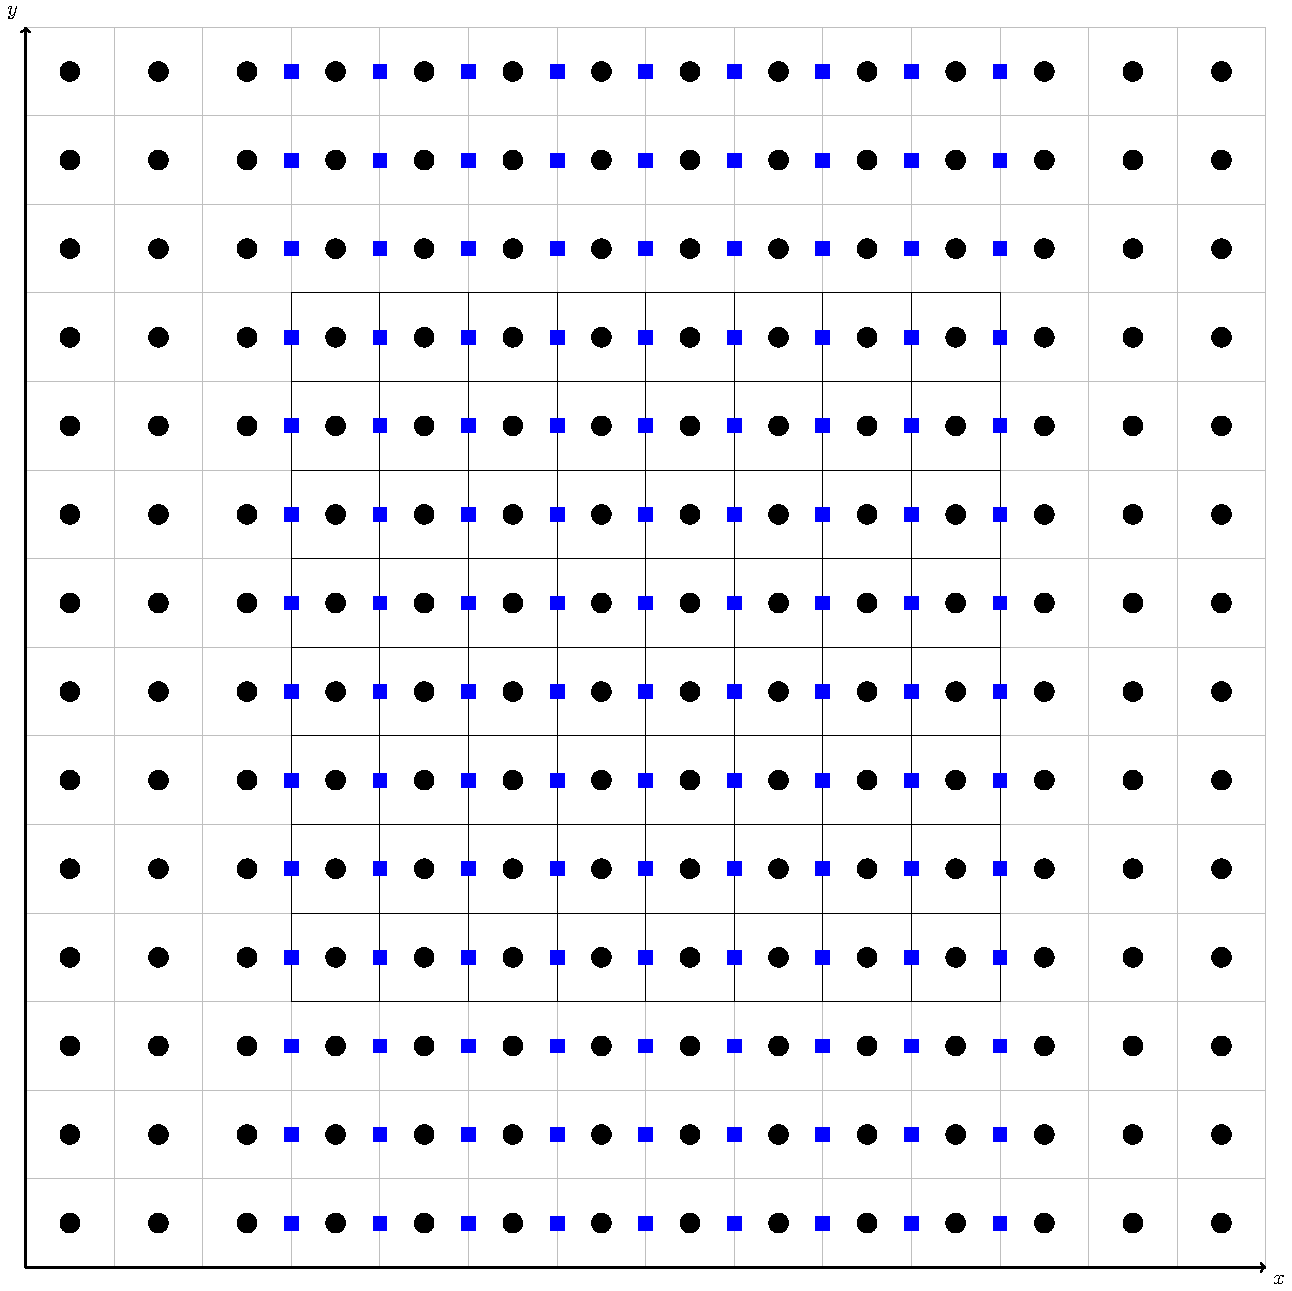
\includegraphics[width=1\linewidth]{2d_grid_Qx}
		\caption{$Q^n$ (black circles) and $u$ at edges (blue squares). \label{lt-Qx}}
	\end{subfigure}
	\begin{subfigure}{0.3\textwidth}
		\centering
		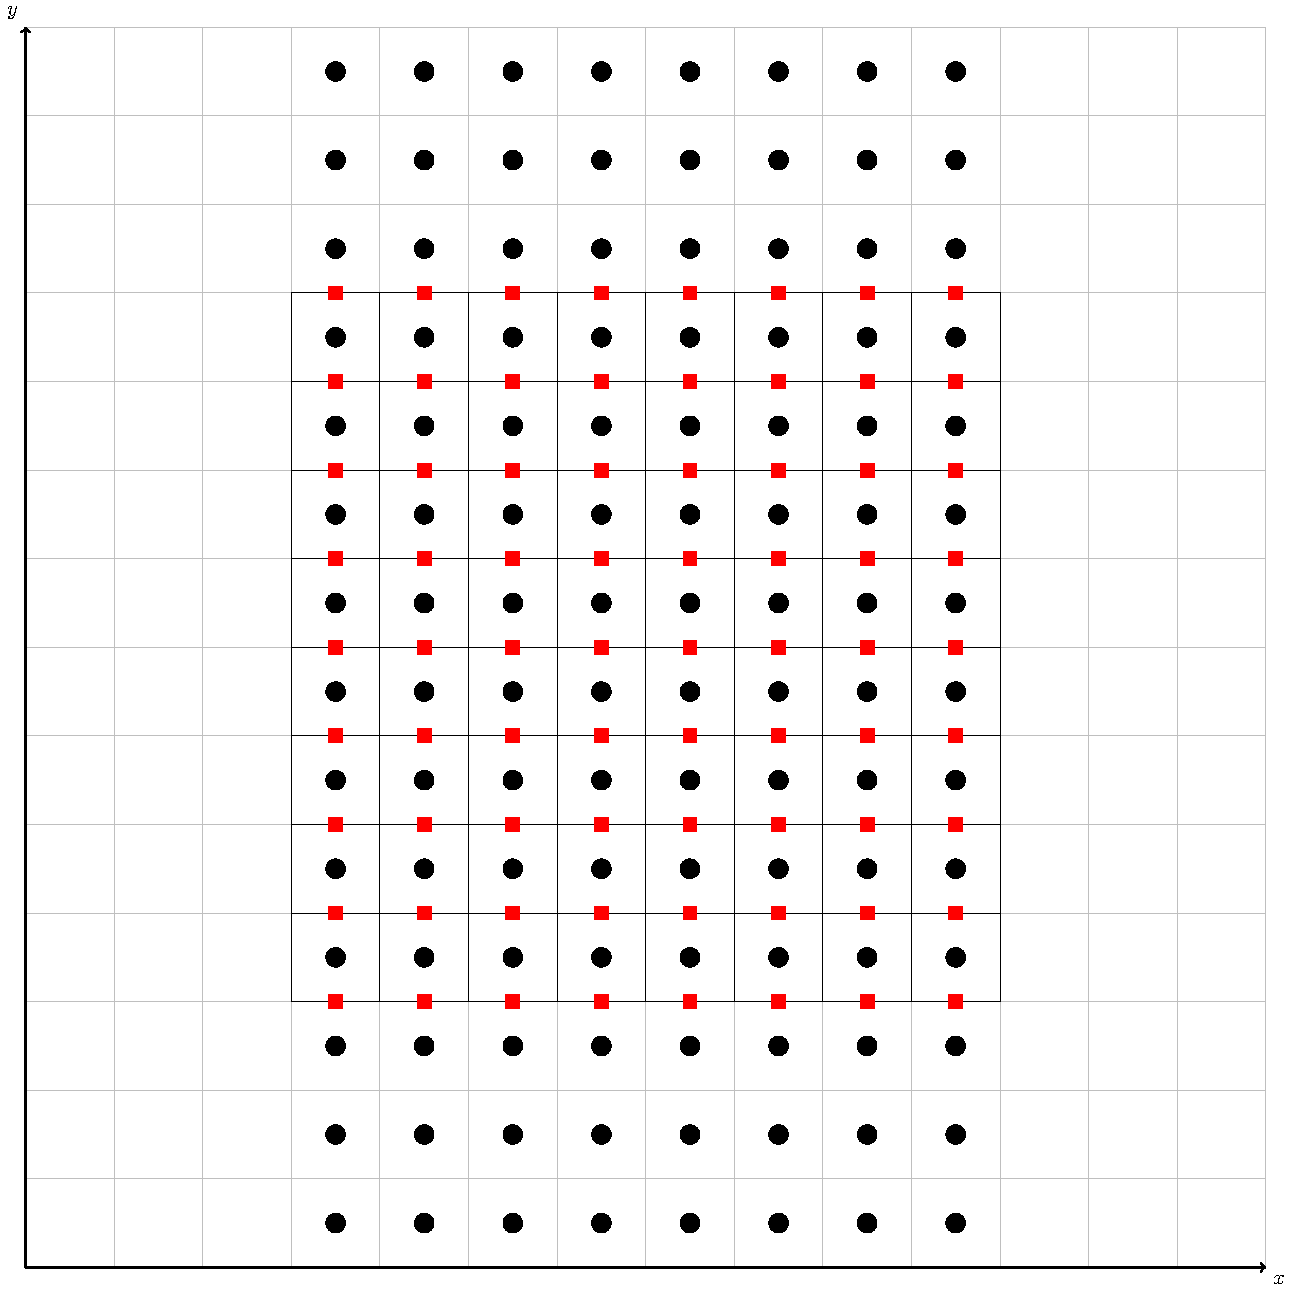
\includegraphics[width=1\linewidth]{2d_grid_FQ}
		\caption{$Q^{x,n}$ (black circles) and $v$ at edges (red squares).\label{lt-FQx} }
	\end{subfigure}
	\begin{subfigure}{0.3\textwidth}
	    \centering
	    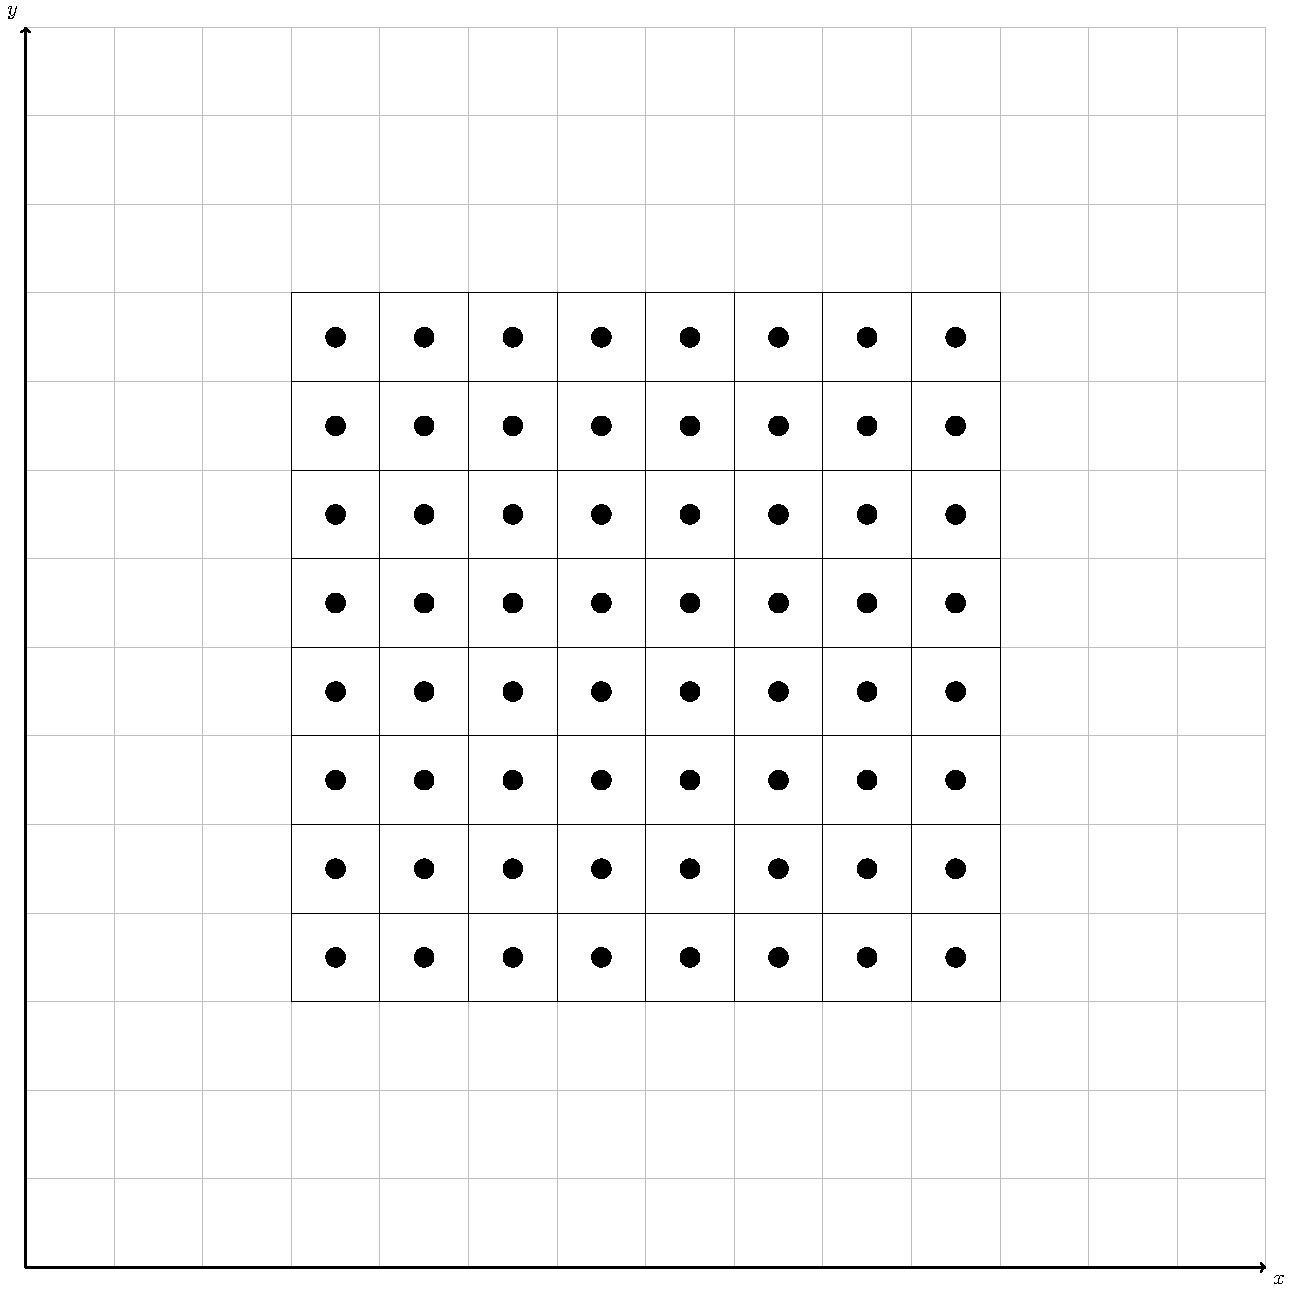
\includegraphics[width=1\linewidth]{2d_grid_GFQ}
		\caption{$Q^{yx,n}$ (black circles) after advecting $Q^{x,n}$ in $y$ direction. \label{lt-GFQx}}
    \end{subfigure}
	\caption{Illustration of the Lie-Trotter splitting applied in the $x$ direction (operator $\mathbf{F}$)
	and then in the $y$ direction (operator $\mathbf{G}$). Interior cells are depicted using black lines,
	 while ghost cells are depicted using gray lines. 
	 All the winds shown are the ones used in the DP1 departure point scheme.
	 If the DP2 scheme is used, an additional layer of wind ghost values should be added at each boundary in (a) and (b). \label{ltxdir}}
\end{figure}


\begin{figure}[!htb]
	\centering
	\begin{subfigure}{0.3\textwidth}
		\centering
		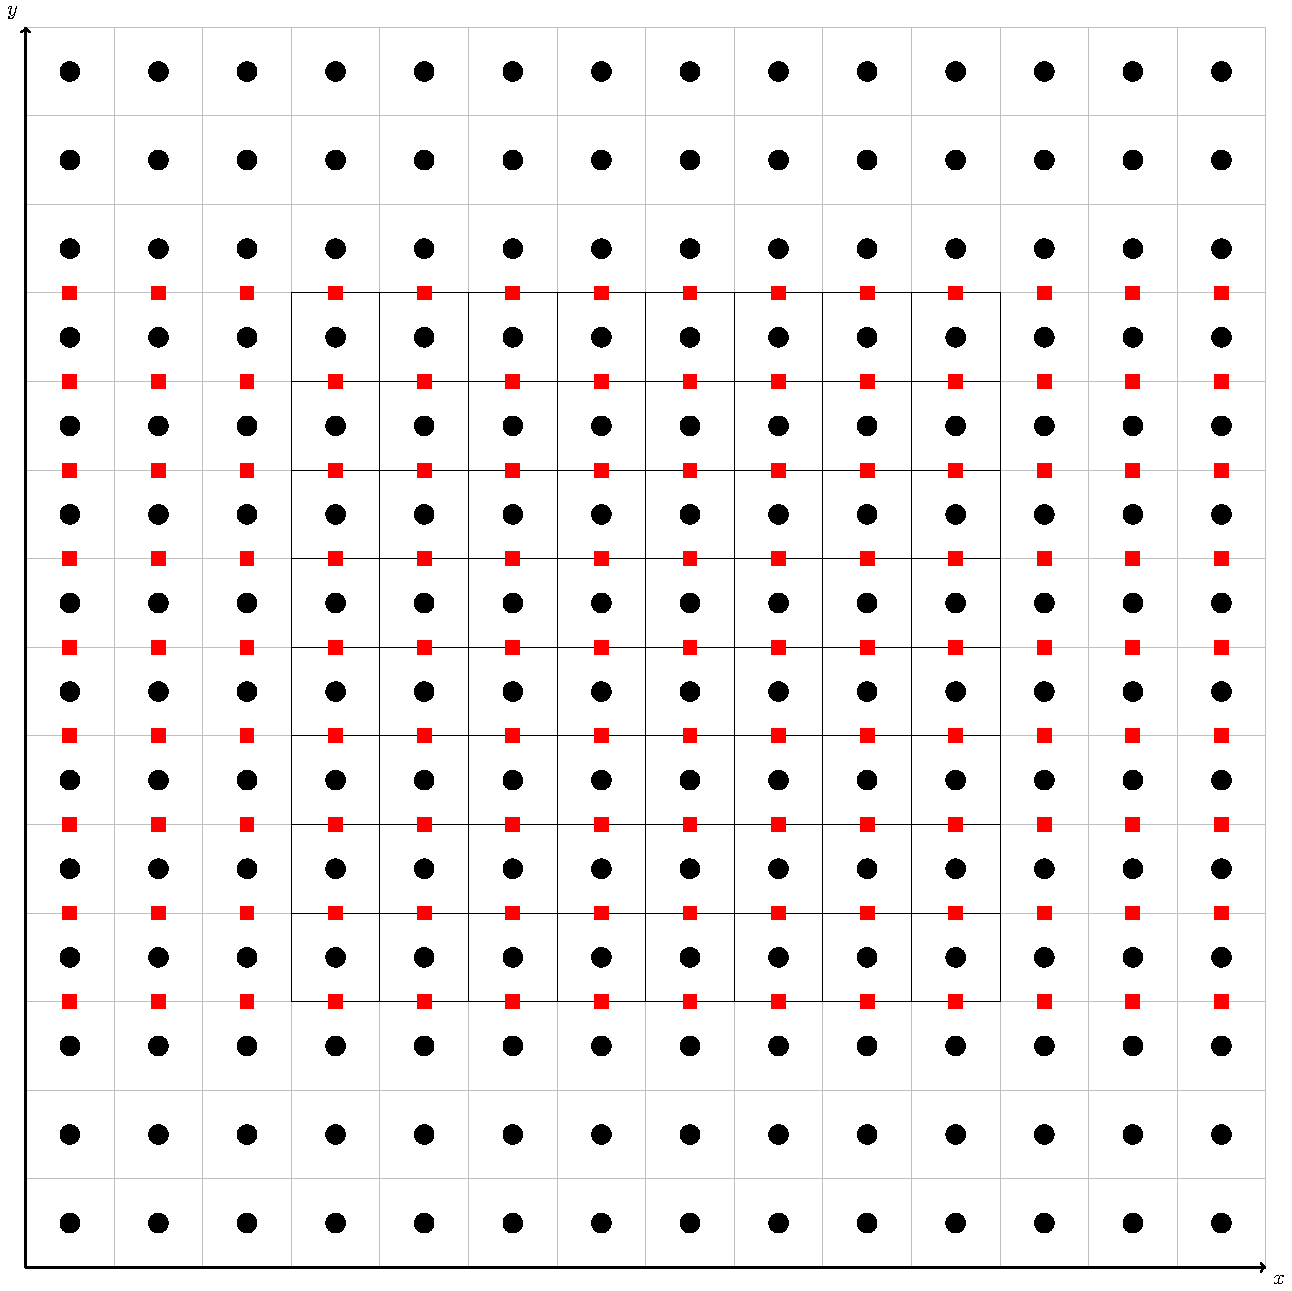
\includegraphics[width=1\linewidth]{2d_grid_Qy}
		\caption{$Q^n$ (black circles) and $v$ at edges (red squares). \label{lt-Qy}}
	\end{subfigure}
	\begin{subfigure}{0.3\textwidth}
		\centering
		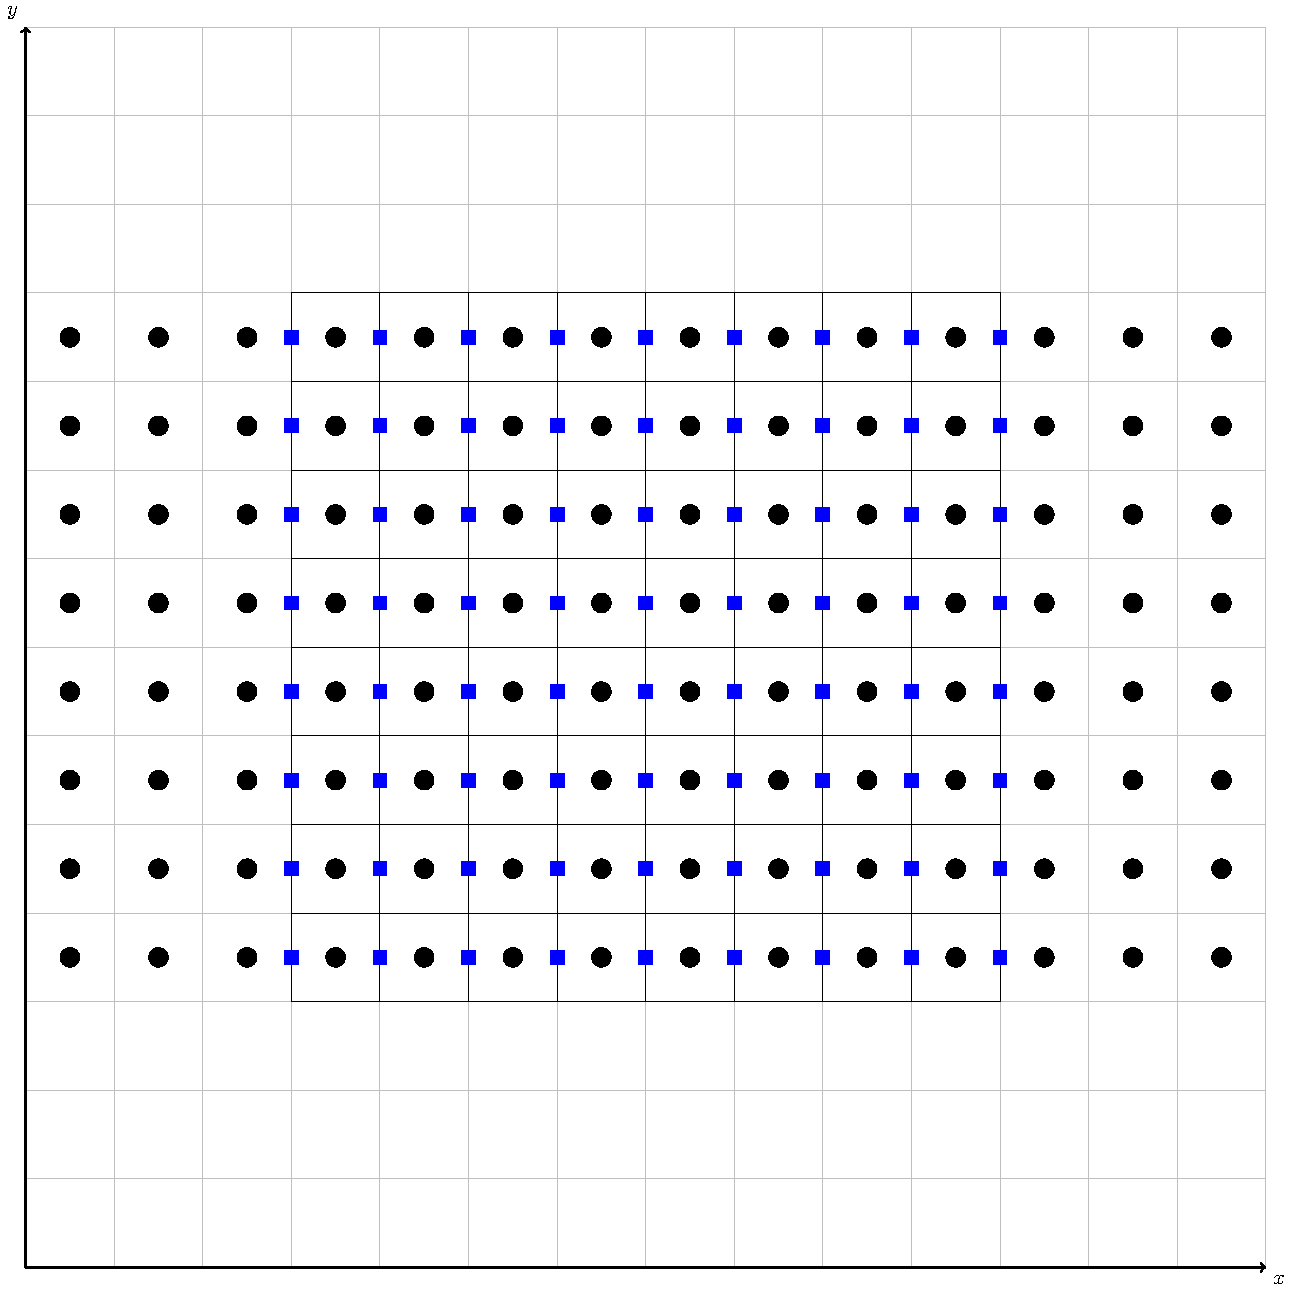
\includegraphics[width=1\linewidth]{2d_grid_GQ}
		\caption{$Q^{y,n}$ (black circles) and $u$ at edges (blue squares).\label{lt-GQy} }
	\end{subfigure}
	\begin{subfigure}{0.3\textwidth}
		\centering
		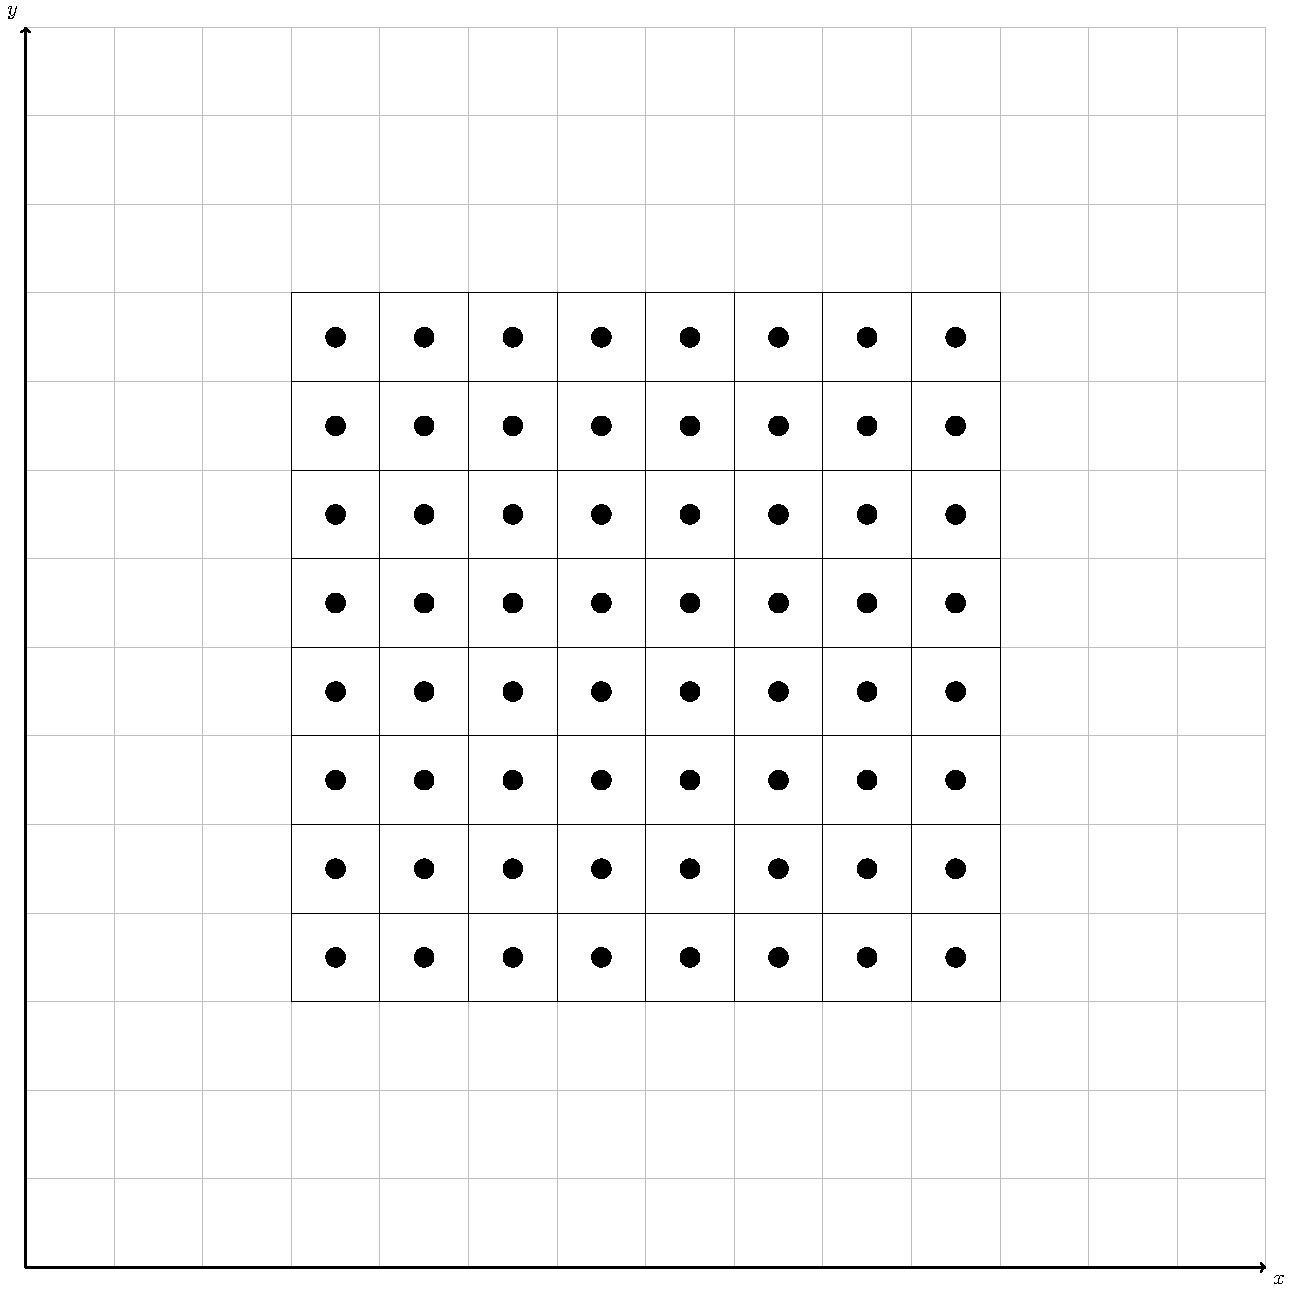
\includegraphics[width=1\linewidth]{2d_grid_GFQ}
		\caption{$Q^{xy,n}$ (black circles) after advecting $Q^{y,n}$ in $x$ direction. \label{lt-FGQy}}
	\end{subfigure}
	\caption{Similar to Figure \ref{ltxdir} but considering the Lie-Trotter splitting in reverse order.}
\end{figure}

The Lie-Trotter splitting is obtained by solving the advection in the $x$ direction
\begin{align*}
	{Q}^{x,n}_{ij} =  {Q}^{n}_{ij} + \mathbf{F}_{ij}[{Q^n}, \tilde{c}^{x,n}],
\end{align*}
for $j=\nu+1, \ldots, M+\nu$, $i=1, \ldots, N$ (Figure \ref{lt-FQx}), and then we advect in the $y$ direction with initial data ${Q}^{x,n}$ 
\begin{align*}
	{Q}^{yx,n}_{ij} = Q^{x,n}_{ij} + \mathbf{G}_{ij}[{Q}^{x,n},\tilde{c}^{y,n}],
\end{align*}
for $j=1, \ldots, M$,  $i=1, \ldots, N$  (Figure \ref{lt-GFQx}).
To get the average Lie-Trotter splitting we repeat the process in the reverse order by solving the advection equation
in the $y$ direction
\begin{align*}
	{Q}^{y,n}_{ij} =  {Q}^{n}_{ij} + \mathbf{G}_{ij}[{Q^n},\tilde{c}^{y,n}],
\end{align*}
for $i=-\nu+1, \ldots, N+\nu$, $j=1, \ldots, M$ (Figure \ref{lt-GQy}), and then we advect in the $x$-direction with initial data ${Q}^{y,n+1}$ 
\begin{align*}
	{Q}^{xy,n}_{ij} = Q^{y,n}_{ij} + \mathbf{F}_{ij}[Q^{y,n},\tilde{c}^{x,n}],
\end{align*}
for $i=1, \ldots, N$, $j=1, \ldots, M$ (Figure \ref{lt-FGQy}) and thus we have the average Lie-Trotter solution:
\begin{align}
\label{chp-adv2d-LT}
    Q^{n+1} = \frac{(Q^{xy,n} + Q^{yx,n})}{2} 
    = Q^n &+ \frac{1}{2}\mathbf{F}[Q^n,\tilde{c}^{x,n}] + \frac{1}{2}\mathbf{G}[Q^n,\tilde{c}^{y,n}] \nonumber \\
    &+\frac{1}{2}\mathbf{F}\bigg[Q^n + \mathbf{G}[Q^n, \tilde{c}^{y,n}], \tilde{c}^{x,n}\bigg]+
    \frac{1}{2}\mathbf{G}\bigg[Q^n + \mathbf{F}[Q^n, \tilde{c}^{x,n}], \tilde{c}^{y,n}\bigg].
\end{align}
This scheme shall be referred to in this work as the average Lie-Trotter (\textbf{LT}) scheme. 
Finally, we point out that this scheme could be built using any other 1D numerical flux function, 
but we focus on PPM since this is what is used in FV3.
\subsection{Elimination of splitting error for a constant scalar field and non-divergent wind}
Let us, for an instant, assume that $\mathbf{F}$ and $\mathbf{G}$ are linear in their first input. This implies that Equation \eqref{chp-adv2d-LT} may be rewritten as:
\begin{align}
\label{chp-adv2d-LT-linear}
    Q^{n+1} = Q^n 
    &+ \mathbf{F}[Q^n,\tilde{c}^{x,n}] + \mathbf{G}[Q^n,\tilde{c}^{y,n}] \nonumber \\
    &+\frac{1}{2}\mathbf{F}\bigg[\mathbf{G}[Q^n, \tilde{c}^{y,n}], \tilde{c}^{x,n}\bigg]+
      \frac{1}{2}\mathbf{G}\bigg[\mathbf{F}[Q^n, \tilde{c}^{x,n}], \tilde{c}^{y,n}\bigg].
\end{align}
The numerical flux functions defined in Chapter \ref{chp-1d-fv} are indeed linear in the input $Q$ if there are no monotonic constraints,
that is, when we use hord0,
implying that $\mathbf{F}$ and $\mathbf{G}$ are both linear in this case.
%citet{lin:1996} suggests using Equation \eqref{chp-adv2d-LT-linear}
%instead of \eqref{chp-adv2d-LT} to save computational operations, but the current implementation of FV3 does not follow this approach.
We are going to consider Equation \eqref{chp-adv2d-LT-linear}
even when there are monotonic constraints, to analyse the scheme when $\boldsymbol{u}$ is non-divergent ($\nabla \cdot 
\boldsymbol{u} = 0$) and the
scalar field is equal to a constant $\overline{q}$.
Then the solution remains constant. 
Since the wind is non-divergent, it follows from the Helmholtz decomposition theorem 
that there exists a stream function $\psi \in \mathcal{C}^2$ such that
\begin{align*}
    u(x,y,t) &= -\partial_y \psi(x,y,t),\\
    v(x,y,t) &= \partial_x \psi(x,y,t).
\end{align*}
Then, we may compute the wind using centered-finite differences 
\begin{align*}
    u_{i+\frac{1}{2},j}^{n}&=
    -\bigg(\frac{\psi_{i+\frac{1}{2},j+\frac{1}{2}}^{n}-\psi_{i+\frac{1}{2},j-\frac{1}{2}}^{n}}{\Delta y}\bigg),\\
    v_{i,j+\frac{1}{2}}^{n} &= 
    \frac{\psi_{i+\frac{1}{2},j+\frac{1}{2}}^{n}-\psi_{i-\frac{1}{2},j+\frac{1}{2}}^{n}}{\Delta x},\\
\end{align*}
and thus the following discrete divergence free condition holds
\begin{align}
\label{discrete-divfree}
  \frac{\delta_i u_{ij}^n}{\Delta x} + \frac{\delta_j v_{ij}^n}{\Delta y} = 0.
\end{align}
Notice that this identity holds for the time-averaged winds if we assume that
that $\tilde{u}^n$ and  $\tilde{v}^n$ are computed using DP1.
If we use DP2, this identity is no longer valid.
Now, using the fact that the scalar field is supposed to be constant, we have:
\begin{align*}
\mathbf{F}_{ij}[\overline{q},\tilde{c}^{x,n}] &= -\overline{q} \lambda \delta_i \tilde{u}_{ij}^n,\\
\mathbf{G}_{ij}[\overline{q},\tilde{c}^{y,n}] &= -\overline{q} \lambda \delta_j \tilde{v}_{ij}^n,
\end{align*}
recalling that $\lambda = \frac{\Delta t}{\Delta x} = \frac{\Delta t}{\Delta y}$.
Applying $\mathbf{G}$ and $\mathbf{F}$ again, we have:
\begin{align*}
\mathbf{G}_{ij}\big[\mathbf{F}[{\overline{q},\tilde{c}^{y,n}}],\tilde{c}^{x,n}\big] &= 
   \overline{q}\lambda^2 \bigg(
   \tilde{v}_{i,j+\frac{1}{2}}^n\mathfrak{F}_{i,j+\frac{1}{2}}^{PPM,y}[ {\delta_i} \tilde{u}_{ij}^n,\tilde{c}^{y,n}] 
-  \tilde{v}_{i,j-\frac{1}{2}}^n\mathfrak{F}_{i,j-\frac{1}{2}}^{PPM,y}[ {\delta_i} \tilde{u}_{ij}^n,\tilde{c}^{y,n}]\bigg)\\
&=  \overline{q}\lambda^2\delta_i \big( \tilde{v}_{ij}^n\mathfrak{F}_{ij}^{PPM,y}[ {\delta_i} \tilde{u}_{ij}^n,\tilde{c}^{y,n}] \big),
\end{align*}
\begin{align*}
\mathbf{F}_{ij}\big[\mathbf{G}[{\overline{q},\tilde{c}^{x,n}}],\tilde{c}^{y,n}\big] &= 
   \overline{q}\lambda^2 \bigg(
   \tilde{u}_{i,j+\frac{1}{2}}^n\mathfrak{F}_{i,j+\frac{1}{2}}^{PPM,x}[ {\delta_j} \tilde{v}_{ij}^n,\tilde{c}^{x,n}] 
-  \tilde{u}_{i,j-\frac{1}{2}}^n\mathfrak{F}_{i,j-\frac{1}{2}}^{PPM,x}[ {\delta_j} \tilde{v}_{ij}^n,\tilde{c}^{x,n}] \bigg)\\
&=  \overline{q}\lambda^2\delta_j \big( \tilde{u}_{ij}^n\mathfrak{F}_{ij}^{PPM,x}[ {\delta_j} \tilde{v}_{ij}^n,\tilde{c}^{x,n}] \big).
\end{align*}
However, if we compute the updated solution using Equation \eqref{chp-adv2d-LT-linear} we have that the error is given by
\begin{align}
	\label{chp-adv2d-LT-error}
	Q^{n+1}_{ij} - \overline{q} &= 
	-\Delta t \bigg(\frac{\delta_i \tilde{u}_{ij}^n}{\Delta x} + \frac{\delta_j \tilde{v}_{ij}^n}{\Delta y} \bigg)
	-\frac{\overline{q}}{2}\lambda^2
	\bigg(
	\delta_j \big( \tilde{u}_{ij}^n\mathfrak{F}_{ij}^{PPM,x}[ {\delta_j} \tilde{v}_{ij}^n,\tilde{c}^{x,n}] \big)+
        \delta_i \big( \tilde{v}_{ij}^n\mathfrak{F}_{ij}^{PPM,y}[ {\delta_i} \tilde{u}_{ij}^n,\tilde{c}^{y,n}] \big)\bigg) \nonumber\\
	&=
	-\frac{\overline{q}}{2}\lambda^2
	\bigg(
	\delta_j \big( \tilde{u}_{ij}^n\mathfrak{F}_{ij}^{PPM,x}[ {\delta_j} \tilde{v}_{ij}^n,\tilde{c}^{x,n}] \big)+
        \delta_i \big( \tilde{v}_{ij}^n\mathfrak{F}_{ij}^{PPM,y}[ {\delta_i} \tilde{u}_{ij}^n,\tilde{c}^{y,n}] \big)\bigg),
\end{align}
To eliminate this error, \citet{lin:1996} proposed modifying the Equation \eqref{chp-adv2d-LT} to
\begin{align}
\label{chp-adv2d-PL}
Q^{n+1} = Q^n &+ \frac{1}{2}\mathbf{F}[Q^n,\tilde{c}^{x,n}] + \frac{1}{2}\mathbf{G}[Q^n,\tilde{c}^{y,n}]\nonumber \\
&+\frac{1}{2}\mathbf{F}\bigg[Q^n + \mathbf{g}[Q^n, \tilde{c}^{y,n}], \tilde{c}^{x,n}\bigg]+
\frac{1}{2}\mathbf{G}\bigg[Q^n + \mathbf{f}[Q^n, \tilde{c}^{x,n}], \tilde{c}^{y,n}\bigg],
\end{align}
where $\mathbf{f}$ and $\mathbf{g}$ are called inner advective operators.
In this work, we shall consider the inner advective operator proposed by \citet{putman:2007} (hereafter referred to as \textbf{PL}).
The PL scheme is currently used in the FV3 dynamical core. Also, notice that the LT scheme is equivalent to the PL scheme but uses 
$\mathbf{f}=\mathbf{F}$ and $\mathbf{g}=\mathbf{G}$.
All the expressions for each inner advective operator mentioned are shown in Table \ref{chp-adv2d-tab1}.
\begin{table}[!h]
	\begin{tabular}{|c|l|l|}
		\hline
		Scheme & \multicolumn{1}{c|}{$\mathbf{f}_{ij}(Q^n, \tilde{c}^{x,n})$}
		       & \multicolumn{1}{c|}{$\mathbf{g}_{ij}(Q^n, \tilde{c}^{y,n})$} \\ \hline
		LT   & $\mathbf{F}_{ij}(Q^n,\tilde{c}^{x,n})$ 
		       & $\mathbf{G}_{ij}(Q^n,\tilde{c}^{y,n})$ \\ \hline
		PL   & $-Q_{ij}^n +
		         \frac{Q_{ij}^n  + \mathbf{F}_{ij}(Q^n,\tilde{c}^{x,n})}
			   {1 - \frac{1}{|\Omega_{ij}|}\big(\mathcal{A}_{i+\frac{1}{2},j}^{x} - \mathcal{A}_{i-\frac{1}{2},j}^{x}\big)}$
			   & $-Q_{ij}^n +
			 \frac{Q_{ij}^n  + \mathbf{G}_{ij}(Q^n,\tilde{c}^{y,n})}
			   {1 - \frac{1}{|\Omega_{ij}|}\ \big(\mathcal{A}_{i,j+\frac{1}{2}}^{y} - \mathcal{A}_{i,j-\frac{1}{2}}^{y}\big)}$
			   \\ \hline
	\end{tabular}
\caption{Expression of the inner advective operators considered in this work.
LT stands for the average Lie-Trotter  scheme, while PL stands for the scheme from \citet{putman:2007}.}
\label{chp-adv2d-tab1}
\end{table}
It is easy to see that the PL operator eliminates the term multiplied by $\lambda^2$ that appeared in Equation \eqref{chp-adv2d-LT-error}
when we apply these operators to a constant grid function $Q^n$ and a non-divergent velocity field in Equation \eqref{chp-adv2d-LT-error}.
Therefore, these inner advective operators eliminate the splitting error for a constant field and a non-divergent velocity field, making this scheme exact in this case
if we use DP1 to compute the departure points.
If we use DP2 with PL splitting, Equation \eqref{chp-adv2d-LT-error} will introduce a first-order error since the discrete divergence-free condition (Equation \eqref{discrete-divfree})
for the time-averaged winds of DP2 does not hold in this case.
We shall see this in the numerical experiments (Section \ref{sec-ds-exp}).
We point out that although the LT scheme has an error in Equation \eqref{chp-adv2d-LT-error}, it is a second-order error,
since this scheme is generally second-order accurate \citep{holden:2010}, provided that the 1D flux is second-order, 
which shall be the case if we use the DP2 scheme as discussed in Chapter \ref{chp-1d-fv}.

\section{Numerical experiments}
\label{sec-ds-exp}
To assess the dimension-splitting schemes LT and PL introduced previously, we are going to consider the linear advection 
equation on the spatial domain $[-\frac{L}{2},\frac{L}{2}]\times[-\frac{L}{2},\frac{L}{2}]$ and in the time interval $[0,T]$, 
with biperiodic boundary conditions, where $L = \frac{\pi}{2} R$. Here, $R = 6.371 \times 10^6$ meters, 
representing the Earth's radius, and $T = 1036800$ seconds, equivalent to 12 days. 
The spatial domain spans approximately $10^4$ kilometers in both directions,
which correspond to approximately the lengths of a cubed-sphere panel,
as shall be seen in Chapter \ref{chp-cs-grids}.

For the 1D schemes, we will consider the FV-SL schemes \textbf{hord0} (Subsection \ref{chp-adv1d-sec-hord0}) and
\textbf{hord8} (Subsection \ref{chp-adv1d-sec-hord8}), 
each tested with both departure point schemes \textbf{DP1} (Subsection \ref{chp-adv1d-sec-DP1}) and \textbf{DP2} (Subsection \ref{chp-adv1d-sec-DP2}).
We employ $(\Delta x^{(k)},\Delta y^{(k)},\lambda)$-discretizations with $\Delta x^{(k)} = \Delta y^{(k)} = \frac{L}{N^{(k)}}$,
$N^{(k)} = 48 \times 2^k$, $k=0,\ldots, 4$.
We introduce the relative error in the maximum norm:
\begin{equation*}
	E_k = 
	\frac{\| Q^n - Q^0 \|_{\infty, \Delta x \times \Delta y}}
	{\|Q^0\|_{\infty, \Delta x \times \Delta y}}.
\end{equation*}
The convergence rate, as defined in Section \ref{chp-adv1d-sec-numerical-exp}, and the preservation of total mass variation with 
machine precision are considered in all experiments presented here.
It is worth noting that in error computation, we employ centroid values instead of exact average values to avoid 
the computation of analytical integrals.
This approximation, as discussed in Proposition \ref{prop-bound-centroid-2d}, introduces a second-order error.

\subsection{Square wave with constant wind advection}
For the initial test, a constant velocity $\boldsymbol{u}=\big(\frac{L}{T},\frac{L}{T}\big)$ is considered.
The IC is a rectangular profile (refer to Figure \ref{chp-adv2d-sec-exp-adv1-a}) given by:
\begin{equation}
	\label{chp-adv2d-ic1}
	q_0(x,y) =  
	\begin{cases}
		1 & \text{if } (x,y) \in [-0.1L,0.1L]\times [-0.1L,0.1L],\\
		0.1 & \text{otherwise}.
	\end{cases}
\end{equation}
\begin{figure}[!htb]
	\centering
	\begin{subfigure}{0.3\textwidth}
		\centering
		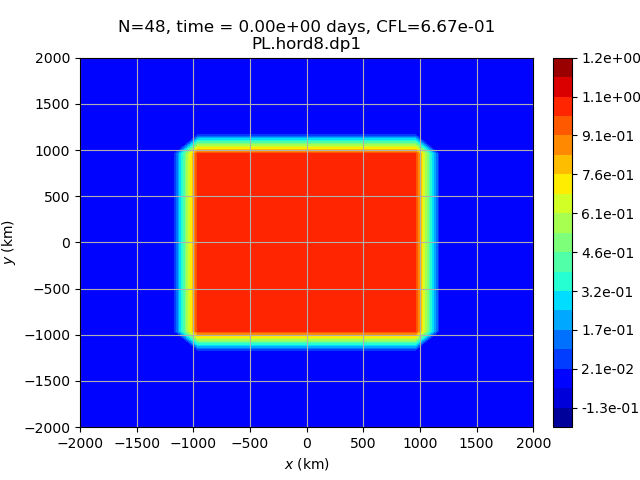
\includegraphics[width=1\linewidth]{adv2d_tc1_N48_hord8_iadv1_dp1_t0}
		\caption{IC\label{chp-adv2d-sec-exp-adv1-a}}
	\end{subfigure}
	\begin{subfigure}{0.3\textwidth}
		\centering
		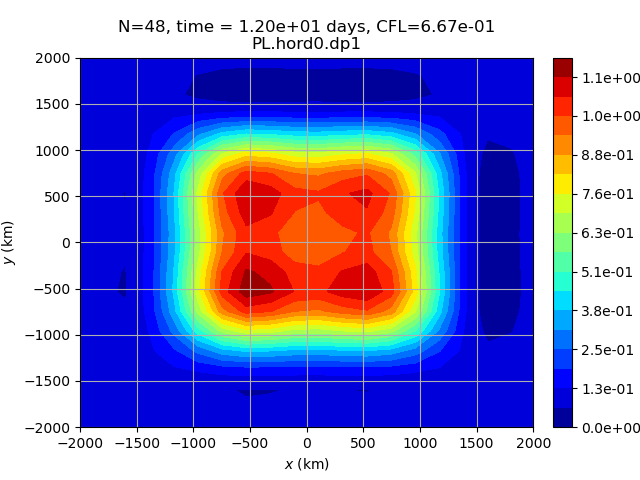
\includegraphics[width=1\linewidth]{adv2d_tc1_N48_hord0_iadv1_dp1_t12}
		\caption{PL-hord0\label{chp-adv2d-sec-exp-adv1-b}}
	\end{subfigure}
	\begin{subfigure}{0.3\textwidth}
		\centering
		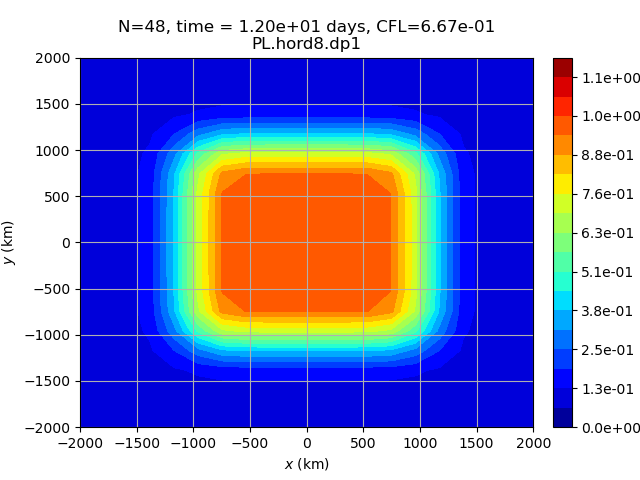
\includegraphics[width=1\linewidth]{adv2d_tc1_N48_hord8_iadv1_dp1_t12}
		\caption{PL-hord8.\label{chp-adv2d-sec-exp-adv1-c}}
	\end{subfigure}	
	\caption{Linear advection experiment using a constant velocity $\boldsymbol{u} = \left(\frac{L}{T},\frac{L}{T}\right)$, 
	a CFL number set to $0.67$, and a grid resolution of $N=M=48$.
	The initial condition is given by Equation \eqref{chp-adv2d-ic1}.
	We run this test with the PL splitting combined with the schemes hord0 (b) and hord8 (c).
        The figures display the advected profile after 12 days (one time period).
        The initial condition is depicted in (a). \label{chp-adv2d-sec-exp-adv1}}
\end{figure}

We will employ a time step of 14400 seconds and set $N=M=48$, resulting in a CFL number approximately equal to 0.67.
The exact solution of Problem \ref{chp-adv2d-sec2-prob1} in this scenario is $q_0((x,y)-\boldsymbol{u}t)$.
Due to the constant velocity field, all splitting schemes introduced in Section \ref{sec-dsplit} are equivalent.
Therefore, we only consider the PL splitting. Additionally, it is evident that the Lie-Trotter splitting is exact in this case 
(see, for example, \cite[p.~202-203]{leveque:1990}), meaning no splitting error is introduced.
For the 1D schemes, we utilize DP1 to compute the departure point, as this scheme is exact when the velocity is constant.

The conclusions drawn from this test closely resemble those of the first 1D test discussed in Section \ref{chp-adv1d-sec-numerical-exp-1}.
This similarity arises because no splitting error is introduced when the velocity remains constant.
Figure \ref{chp-adv2d-sec-exp-adv1-c} illustrates that PL splitting maintains monotonicity, particularly noticeable when using the monotonic 1D scheme hord8.

\subsection{Flow deformation with nondivergent wind}
For a first variable velocity testing, we consider two Gaussian hills given by:
\begin{align}
	\begin{split}
	\label{chp-adv2d-ic2}
	q_0(x,y) = 0.1 + 0.9&\exp\bigg(-10\sin^2 \bigg(\pi \bigg(\frac{x}{L}-0.1\bigg)\bigg)\bigg) \exp\bigg(-10\sin^2 \bigg(\pi \frac{y}{L}\bigg) \bigg)+ \\
	           &\exp\bigg(-10\sin^2 \bigg(\pi \bigg(\frac{x}{L}+0.1\bigg)\bigg)\bigg) \exp\bigg(-10\sin^2 \bigg(\pi \frac{y}{L}\bigg) \bigg),
	\end{split}
\end{align}
defined in $[-\frac{L}{2},\frac{L}{2}] \times [-\frac{L}{2},\frac{L}{2}]$, whose graph is shown in Figure \ref{chp-adv2d-sec-exp-adv2-ic}.
\begin{figure}[!htb]
	\centering
	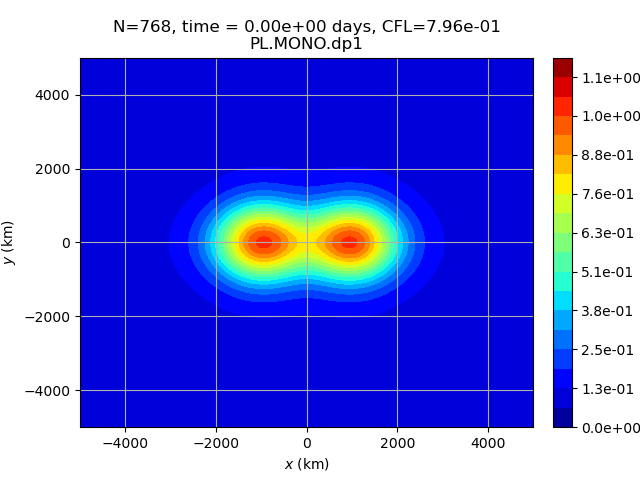
\includegraphics[width=0.5\linewidth]{adv2d_tc3_N768_hord8_iadv1_dp1_t0}
	\caption{Two Gaussian hills IC (Equation \eqref{chp-adv2d-ic2}). \label{chp-adv2d-sec-exp-adv2-ic}}
\end{figure}

We consider the Cartesian version of the deformational flow test case on the sphere from \citet{nair:2010}
proposed by \citet{chen:2017}. The velocity is given by:
\begin{equation}
	\label{chp-adv2d-vf1}
	\begin{cases}
		u(x,y,t) &= -c\frac{L}{T} \sin^2(\alpha_1)\sin\big(\frac{\pi y}{L}\big)\cos\big(\frac{\pi y}{L}\big)  \cos\big(\frac{\pi t}{T}\big) + \frac{L}{T},\\
		v(x,y,t) &= -2c\frac{L}{T}\sin(\alpha_1)  \cos(\alpha_1)\cos^2\big(\frac{\pi y}{L}\big)\cos\big(\frac{\pi t}{T}\big),
	\end{cases}
\end{equation}
where $\alpha_1 = 2\pi\big(\frac{x}{L}-\frac{t}{T}\big)$, $c = 10$.
\citet{chen:2017} uses periodic boundary conditions in the $x-$direction and zero-gradient in the $y-$direction.
However, we will employ biperiodic boundary conditions to simplify the problem.
This velocity field is divergence-free, and deforms the initial condition.
After $T$ time units (12 days in our case), the scalar field returns to its initial position and shape, allowing us to compute the error.
Notice that in Equation \eqref{chp-adv2d-vf1}, we have added a constant wind $\frac{L}{T}$ in the component
$u$ to prevent error cancellation, as discussed by \citet{nair:2010}.

Figure \ref{chp-adv2d-sec-exp-adv2} illustrates the results obtained using two Gaussian hills and the velocity field 
from Equation \eqref{chp-adv2d-vf1}.
We employed a high-resolution grid with $N=768$, along with the PL-DP1-hord8 scheme,
to demonstrate the behavior of the test.
The Figure shows the deformation of the scalar field over time, eventually returning to its initial position.

\begin{figure}[!htb]
	\centering
	\begin{subfigure}{0.25\textwidth}
		\centering
		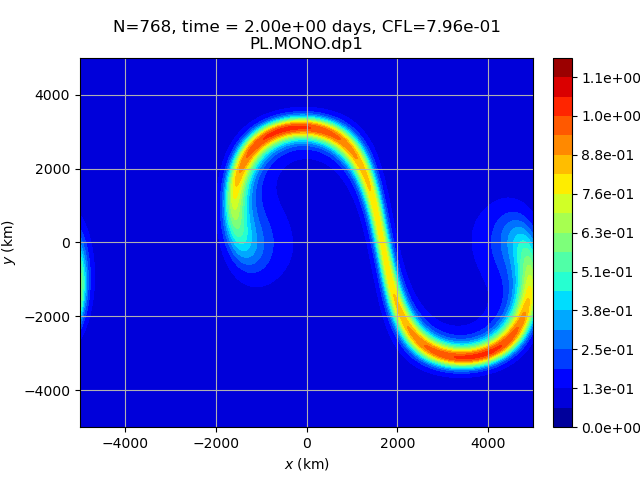
\includegraphics[width=1\linewidth]{adv2d_tc3_N768_hord8_iadv1_dp1_t2}
		\caption{$t=2$.\label{chp-adv2d-sec-exp-adv2-a}}
	\end{subfigure}
	\begin{subfigure}{0.25\textwidth}
		\centering
		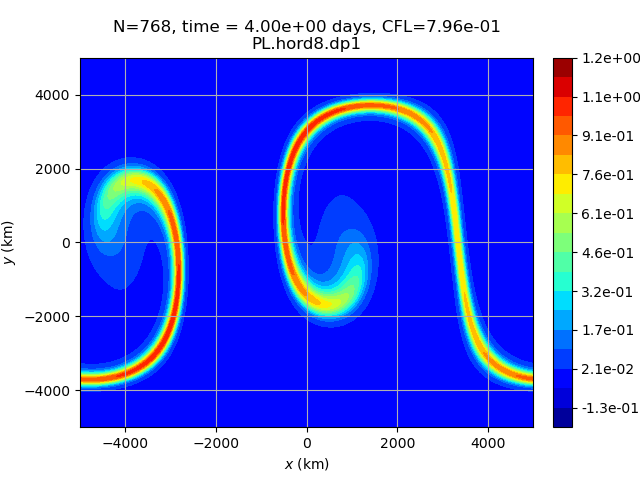
\includegraphics[width=1\linewidth]{adv2d_tc3_N768_hord8_iadv1_dp1_t4}
		\caption{$t=4$ days.\label{chp-adv2d-sec-exp-adv2-b}}
	\end{subfigure}
	\begin{subfigure}{0.25\textwidth}
		\centering
		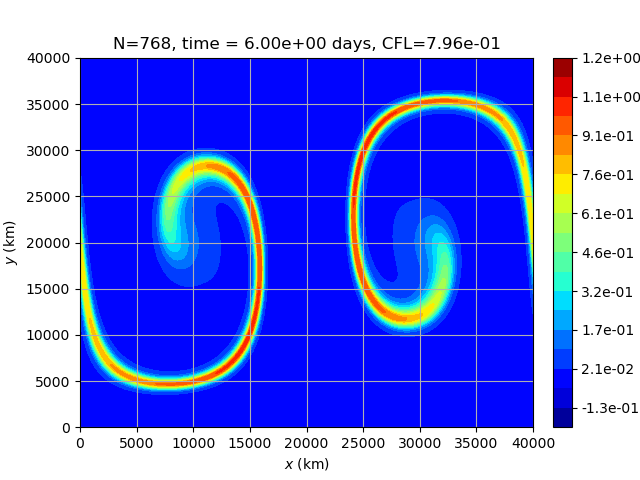
\includegraphics[width=1\linewidth]{adv2d_tc3_N768_hord8_iadv1_dp1_t6}
		\caption{$t=6$ days.\label{chp-adv2d-sec-exp-adv2-c}}
	\end{subfigure}
	
	\begin{subfigure}{0.25\textwidth}
		\centering
		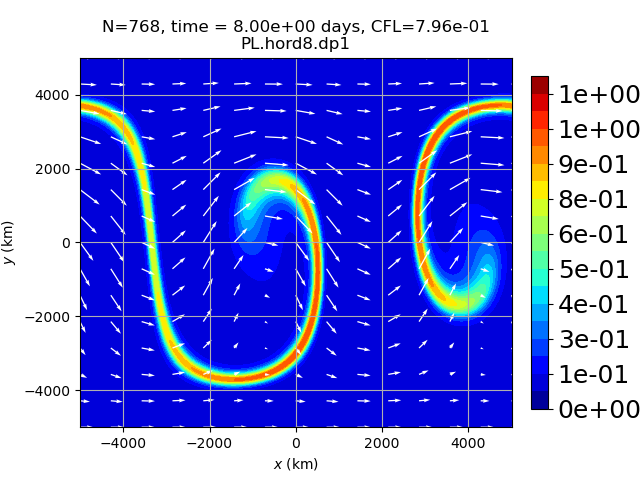
\includegraphics[width=1\linewidth]{adv2d_tc3_N768_hord8_iadv1_dp1_t8}
		\caption{$t=8$ days.\label{chp-adv2d-sec-exp-adv2-d}}
	\end{subfigure}
	\begin{subfigure}{0.25\textwidth}
		\centering
		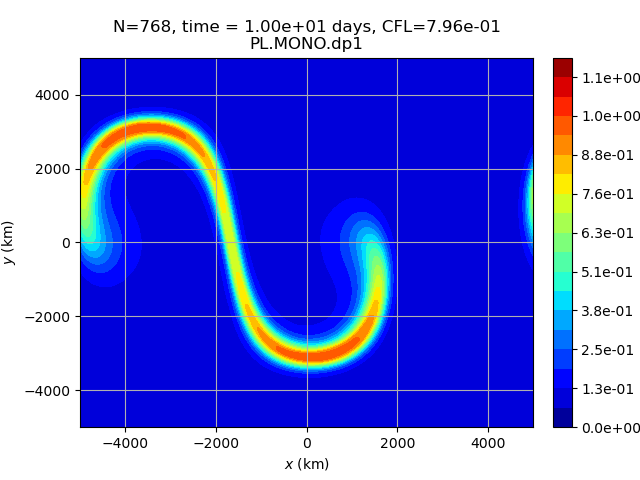
\includegraphics[width=1\linewidth]{adv2d_tc3_N768_hord8_iadv1_dp1_t10}
		\caption{$t=10$ days.\label{chp-adv2d-sec-exp-adv2-e}}
	\end{subfigure}
	\begin{subfigure}{0.25\textwidth}
		\centering
		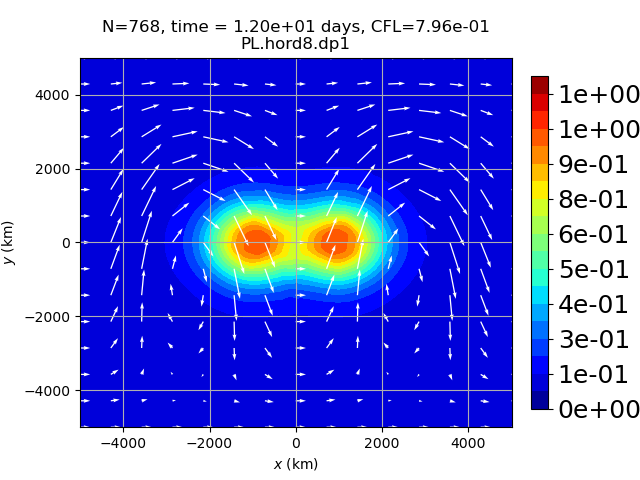
\includegraphics[width=1\linewidth]{adv2d_tc3_N768_hord8_iadv1_dp1_t12}
		\caption{$t=12$ days.\label{chp-adv2d-sec-exp-adv2-f}}
	\end{subfigure}
	\caption{Linear advection experiment using the velocity from Equation \eqref{chp-adv2d-vf1},
		a CFL number equal to $0.79$, $N=768$ cells, and the IC is given by 
		Equation \eqref{chp-adv2d-ic2}
		These figures show the advected profile at
		2 \eqref{chp-adv2d-sec-exp-adv2-a}, 
		4  \eqref{chp-adv2d-sec-exp-adv2-b},
		6  \eqref{chp-adv2d-sec-exp-adv2-c},
		8  \eqref{chp-adv2d-sec-exp-adv2-d},
		10  \eqref{chp-adv2d-sec-exp-adv2-e},
		and 12  \eqref{chp-adv2d-sec-exp-adv2-f} days.
		We are using the PL-DP1-hord8 scheme. \label{chp-adv2d-sec-exp-adv2}}
\end{figure}


\begin{figure}[!htb]
\centering
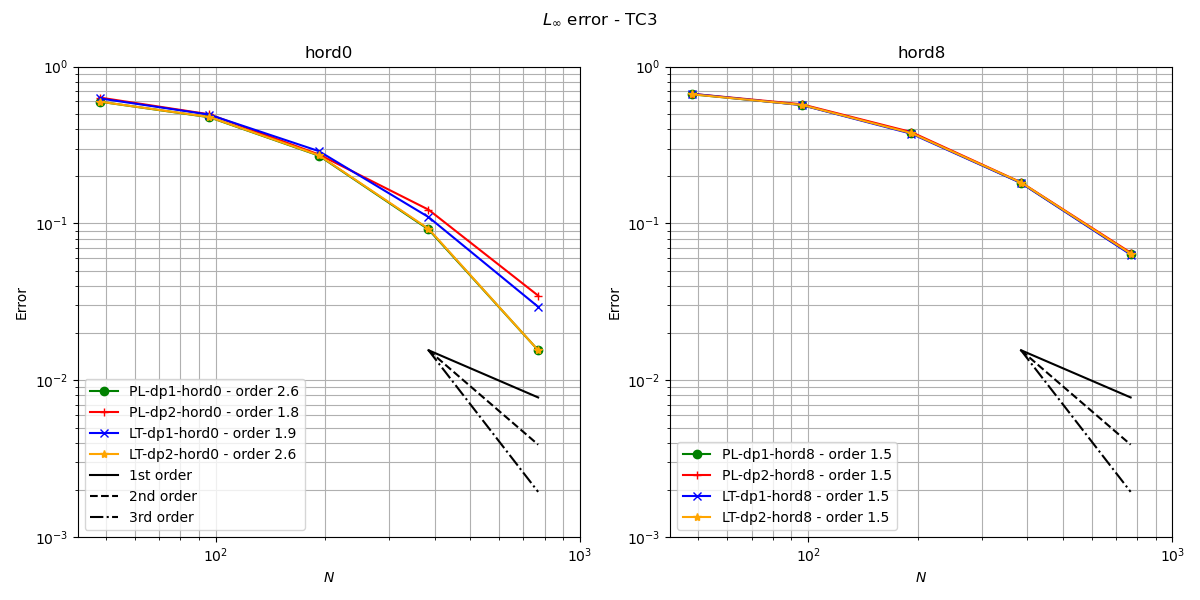
\includegraphics[width=0.67\linewidth]{adv2d_tc3_linf_error}
\caption{$L_{\infty}$ error for the two Gaussian hills (Equation \ref{chp-adv2d-ic2})
with the velocity from Equation \eqref{chp-adv2d-vf1}.
Schemes using hord0 are on the left, and hord8 are on the right.
The PL scheme with DP1 is in green, and with DP2 is in red. 
The LT scheme with DP1 is in blue, and with DP2 is in yellow.
\label{chp-adv2d-sec-exp-adv2-error-linf}}
\end{figure}
\begin{figure}[!htb]
\centering
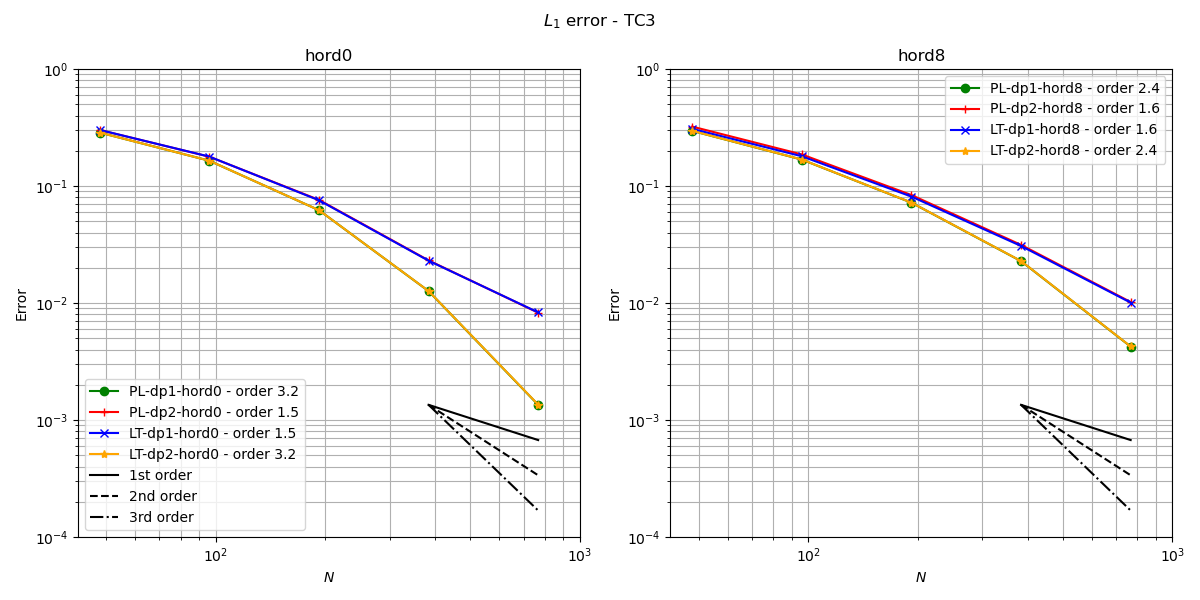
\includegraphics[width=0.67\linewidth]{adv2d_tc3_l1_error}
\caption{Similar to Figure \ref{chp-adv2d-sec-exp-adv2-error-linf} but considering the $L_1$ error.
\label{chp-adv2d-sec-exp-adv2-error-l1}}
\end{figure}

To investigate the error convergence, we employ time steps $\Delta t^{(k)}=\frac{5400}{2^{k}}$ for 
$k = 0, \ldots, 4$, and the spatial discretization as described at the beginning of Section \ref{sec-ds-exp},
resulting in a CFL number approximately equal to 0.79.

We can observe from Figure \ref{chp-adv2d-sec-exp-adv2-error-linf} that for hord0, PL-DP1 and LT-DP2 have smaller
error and higher convergence order than PL-DP2 and LT-DP1.
However, when considering the hord8 scheme, all the schemes have the same error in $L_{\infty}$ norm.
The errors in $L_{1}$ norm (Figure \ref{chp-adv2d-sec-exp-adv2-error-l1}) exhibit a similar behavior; the only difference is 
that PL-DP1 and LT-DP2 have smaller errors than PL-DP2 and LT-DP1, along with higher convergence order.

\subsection{Flow deformation with divergent wind}
For a second variable velocity testing, we consider two Gaussian hills given by Equation 
\eqref{chp-adv2d-ic2} and the following wind:
\begin{equation}
	\label{chp-adv2d-vf2}
	\begin{cases}
		u(x,y,t) &= -\frac{L}{T} \cos^2\big(\frac{\pi x}{L}\big) \sin\big(\frac{2\pi y}{L}\big) \cos\big(\frac{\pi t}{T}\big), \\
		v(x,y,t) &= -\frac{L}{T} \cos^2\big(\frac{\pi y}{L}\big) \sin\big(\frac{2\pi x}{L}\big) \cos\big(\frac{\pi t}{T}\big).
	\end{cases}
\end{equation}
This test is based on the planar test from \citet{nair:2010}, but we adapt it to make the wind divergent.
Figure \ref{chp-adv2d-sec-exp-adv3} illustrates the results obtained using two Gaussian hills and the velocity field 
from Equation \eqref{chp-adv2d-vf2}, similarly to Figure  \ref{chp-adv2d-sec-exp-adv2}.
Again, the IC returns to its initial position after 12 days, allowing us to compute the error.

We employ time steps $\Delta t^{(k)}=\frac{14400}{2^{k}}$ for 
$k = 0, \ldots, 4$, to analyse the error convergence, 
along with the spatial discretization as described at the beginning of Section \ref{sec-ds-exp},
resulting in a CFL number approximately equal to 0.67.
\begin{figure}[!htb]
	\centering
	\begin{subfigure}{0.25\textwidth}
		\centering
		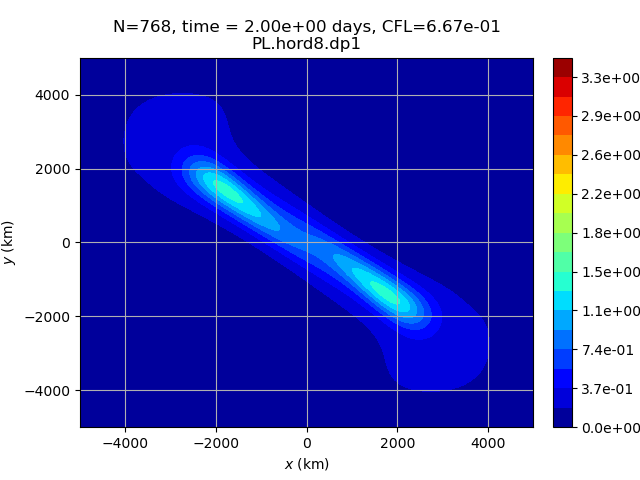
\includegraphics[width=1\linewidth]{adv2d_tc4_N768_hord8_iadv1_dp1_t2}
		\caption{$t=2$.\label{chp-adv2d-sec-exp-adv3-a}}
	\end{subfigure}
	\begin{subfigure}{0.25\textwidth}
		\centering
		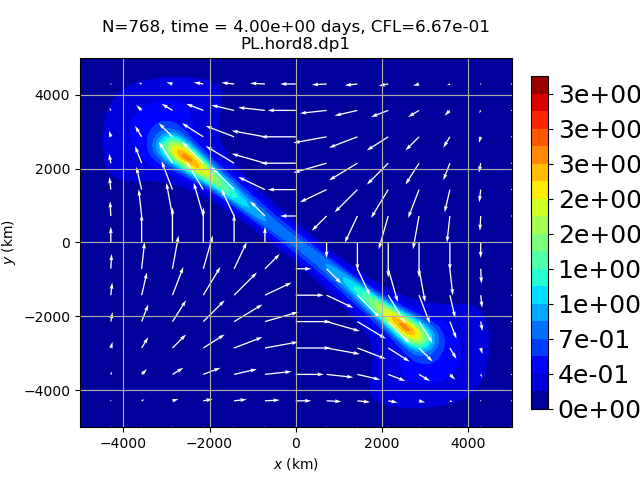
\includegraphics[width=1\linewidth]{adv2d_tc4_N768_hord8_iadv1_dp1_t4}
		\caption{$t=4$ days.\label{chp-adv2d-sec-exp-adv3-b}}
	\end{subfigure}
	\begin{subfigure}{0.25\textwidth}
		\centering
		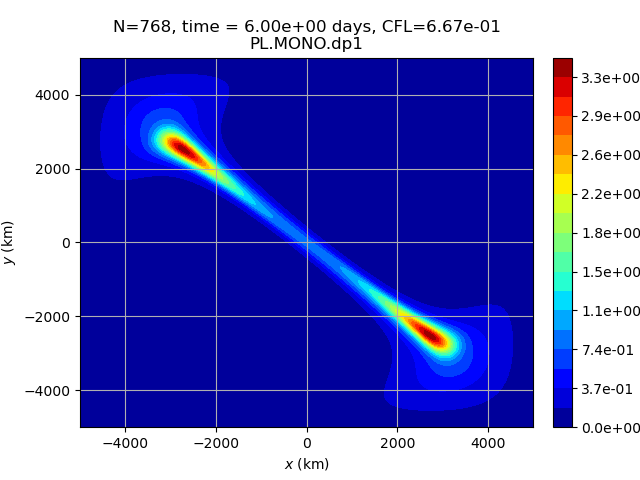
\includegraphics[width=1\linewidth]{adv2d_tc4_N768_hord8_iadv1_dp1_t6}
		\caption{$t=6$ days.\label{chp-adv2d-sec-exp-adv3-c}}
	\end{subfigure}
	
	\begin{subfigure}{0.25\textwidth}
		\centering
		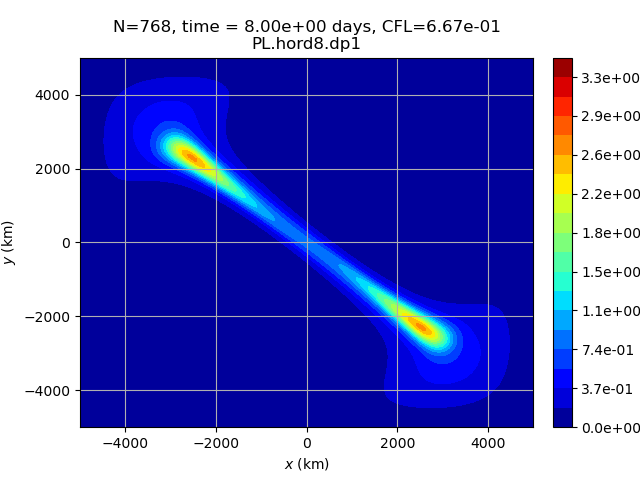
\includegraphics[width=1\linewidth]{adv2d_tc4_N768_hord8_iadv1_dp1_t8}
		\caption{$t=8$ days.\label{chp-adv2d-sec-exp-adv3-d}}
	\end{subfigure}
	\begin{subfigure}{0.25\textwidth}
		\centering
		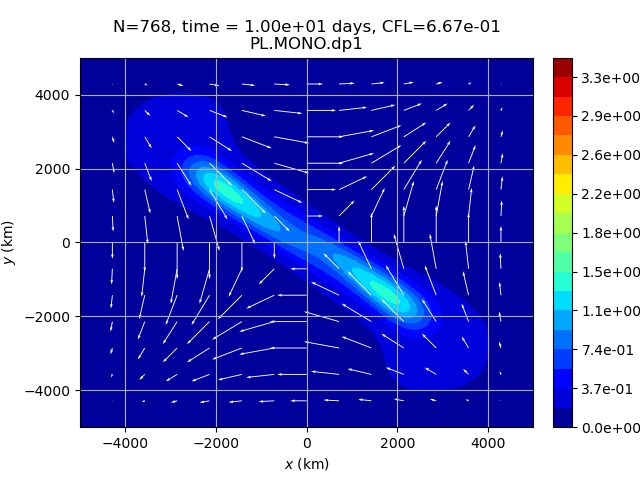
\includegraphics[width=1\linewidth]{adv2d_tc4_N768_hord8_iadv1_dp1_t10}
		\caption{$t=10$ days.\label{chp-adv2d-sec-exp-adv3-e}}
	\end{subfigure}
	\begin{subfigure}{0.25\textwidth}
		\centering
		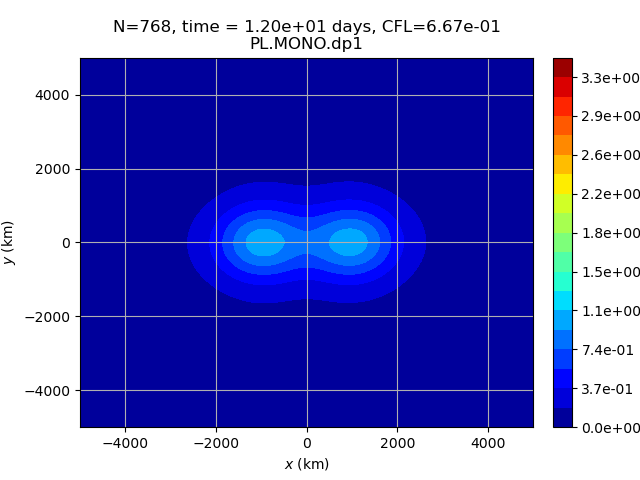
\includegraphics[width=1\linewidth]{adv2d_tc4_N768_hord8_iadv1_dp1_t12}
		\caption{$t=12$ days.\label{chp-adv2d-sec-exp-adv3-f}}
	\end{subfigure}
\caption{Similar to Figure \ref{chp-adv2d-sec-exp-adv2}
but using the wind from Equation \eqref{chp-adv2d-vf2}.\label{chp-adv2d-sec-exp-adv3}}
\end{figure}


\begin{figure}[!htb]
\centering
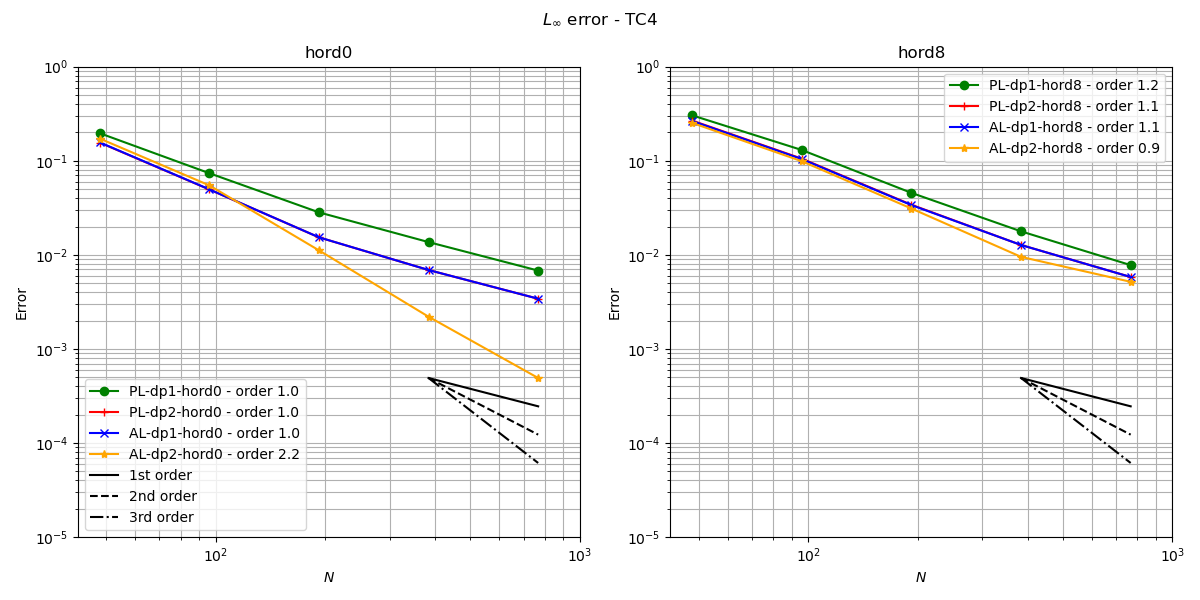
\includegraphics[width=0.67\linewidth]{adv2d_tc4_linf_error}
\caption{Similar to Figure \ref{chp-adv2d-sec-exp-adv2-error-linf}
but using the wind from Equation \eqref{chp-adv2d-vf2}.\label{chp-adv2d-sec-exp-adv3-error-linf}}
\end{figure}

\begin{figure}[!htb]
\centering
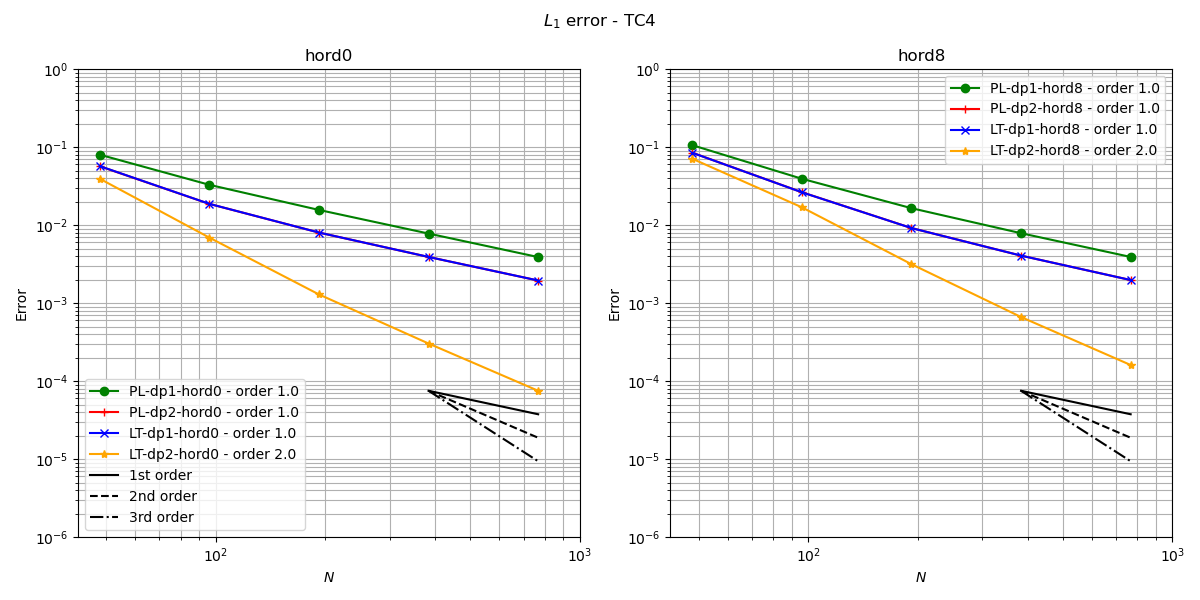
\includegraphics[width=0.67\linewidth]{adv2d_tc4_l1_error}
\caption{Similar to Figure \ref{chp-adv2d-sec-exp-adv3-error-linf} but considering the $L_1$ error.
\label{chp-adv2d-sec-exp-adv3-error-l1}}
\end{figure}

We can observe from Figure \ref{chp-adv2d-sec-exp-adv3-error-linf} that for hord0, PL-DP1 has the bigger error,
while LT-DP2 has the smaller error and the highest convergence rate.
However, when considering the hord8 scheme, all the schemes have almost the same error in $L_{\infty}$ norm.
Regarding the error in $L_{1}$ norm (Figure \ref{chp-adv2d-sec-exp-adv3-error-l1}), we can see that for hord8,
LT-DP2 achieves second-order accuracy, while PL-DP1 achieves only first order.
Finally, the schemes PL-DP2 and LT-DP1 have the same errors for both hord0 and hord8, in both $L_{\infty}$ and $L_{1}$ norms.
%\begin{figure}[!htb]
%	\centering
%	\begin{subfigure}{0.3\textwidth}
%		\centering
%		\includegraphics[width=1\linewidth]{adv2d_tc4_N96_hord8_iadv1_dp2_t0}
%		\caption{IC .\label{chp-adv2d-sec-exp-adv3-2a}}
%	\end{subfigure}
%	\begin{subfigure}{0.3\textwidth}
%		\centering
%		\includegraphics[width=1\linewidth]{adv2d_tc4_N96_hord8_iadv1_dp1_t12}
%		\caption{IC .\label{chp-adv2d-sec-exp-adv3-2a}}
%	\end{subfigure}
%	\begin{subfigure}{0.3\textwidth}
%		\centering
%		\includegraphics[width=1\linewidth]{adv2d_tc4_N96_hord8_iadv1_dp2_t12}
%		\caption{IC .\label{chp-adv2d-sec-exp-adv3-2a}}
%	\end{subfigure}
%	\begin{subfigure}{0.3\textwidth}
%		\centering
%		\includegraphics[width=1\linewidth]{adv2d_tc4_N96_hord8_iadv2_dp1_t12}
%		\caption{IC .\label{chp-adv2d-sec-exp-adv3-2a}}
%
%	\begin{subfigure}{0.3\textwidth}
%		\centering
%		\includegraphics[width=1\linewidth]{adv2d_tc4_N96_hord8_iadv2_dp2_t12}
%		\caption{IC .\label{chp-adv2d-sec-exp-adv3-2a}}
%	\end{subfigure}
%	\caption{ok \label{chp-adv2d-sec-exp-adv3-2}}
%\end{figure}


\section{Concluding remarks}
In this Chapter, we introduced the dimension-splitting method, 
which replaces the solution of the 2D advection equation with the
solution of multiple 1D advection equations, resulting in more cost-effective 2D-FV schemes. 
For our simulations, we adopted the 1D FV-SL scheme based on PPM to solve the 1D equations.

We modified the average of two Lie-Trotter splittings, which is second-order accurate, 
to ensure the preservation of a constant scalar field with a divergence-free velocity,
following the works of \citet{lin:1996} and \citet{putman:2007}.
This modification addresses the limitation of the classical averaging Lie-Trotter splitting and follows the methodology used in FV3.

Based on the simulation with constant velocity, we concluded that all the splitting schemes
are equivalent and do not introduce any splitting errors. In fact, the splittings are exact in this case.
We observed that all the conclusions from the 1D simulations hold true in the 2D case as well,
with mass conservation and monotonicity being preserved when using the monotonic limiters in the 1D subproblems.

In the simulation with variable velocity, we conducted two flow deformation test cases.
For the divergence-free test, the schemes PL-DP1 and LT-DP2 showed similar behavior and performed better
than PL-DP2 and LT-DP1 in all error metrics analyzed here.
However, for the velocity with non-zero divergence, we observed that the scheme PL-DP1 achieved only
first-order accuracy and had larger errors than PL-DP2 and LT-DP1.
This limitation is because the PL-DP1 method is designed to be accurate for divergence-free winds.
This test highlights this limitation because we have divergence.
The scheme LT-DP2 showed better error performance, achieving second-order accuracy regardless of the non-divergence-free condition in the wind.
LT-DP2 also showed second-order accuracy in the $L_1$ norm when we employed the monotonic 1D flux, while PL-DP1 achieved first order.

In summary, the scheme PL-DP1, which is currently used in FV3 as the 2D advection solver, 
showed second-order accuracy for divergence-free winds, with LT-DP2 exhibiting similar behavior. 
However, for non-divergent free winds, LT-DP2 demonstrated second-order accuracy, while PL-DP1 achieved only first order.
